\section{Simulating Quantum Circuits with Pauli-\limdds}
\label{sec:quantum-simulation}

%\todo[inline]{
%-- Prune this overview, referring to Table 2.
%
%-- IMPORTANT: Invent a way to portray the complexities in Table 2 more fairly:\\
% Note that for states/circuits where
% LIMDDs/QMDDs take exponential time, so do ADD (because of their size)! The current caption is not sufficient!
% }

In this section, we give all the algorithms that are necessary to analyze and simulate a quantum circuit with Pauli-\limdds (we will simply say \limdd from now on).
We provide algorithms for dedicated gates, but also an algorithm to apply any multi-qubit gate that is represented as a \limdd.
We also give the subroutine \makeedge which is used to keep the diagram reduced throughout the computation, thus preventing the creation of redundant nodes, keeping the diagram small and canonical. The procedure is the counterpart of `MakeNode' used in other DD definitions for that purpose.
\autoref{tab:complexity} provides an overview of the \limdd algorithms and their 
complexities compared to ADDs and QMDDs (an unequal comparison due to the exponential differences in conciseness shown in \autoref{sec:exponential-separations}).

%In \autoref{sec:equality}, we give a polynomial-time algorithm which checks whether two given \limdds represent the same quantum state.
%In \autoref{sec:measurement}, we give a linear-time algorithm which simulates a measurement performed on the state represented by a \limdd.
%We show both how to compute the probability of observing a given measurement outcome, and how to update the \limdd after a given measurement.
%That is, given a \limdd representing a matrix $U$, and a \limdd representing a state $\ket{\phi}$, \autoref{alg:apply-gate-limdd-limdd} constructs a new \limdd representing the state $U\ket{\phi}$.
%For sake of exposition, we first describe how to apply certain simple gates such as Pauli gates and the Hadamard gate, in \autoref{sec:simple-gates}.
%Lastly, \autoref{sec:makeedge} describes the subroutine \makeedge which is used to keep the diagram reduced throughout the computation, thus preventing the creation of redundant nodes keeping the diagram small and canonical. The procedure is the counterpart of `MakeNode' used in other DD definitions for that purpose.

%\todo[inline]{fix Hadamard for stabilizers}

%\begin{wrapfigure}{r}{5cm}
%        \begin{tikzpicture}[
%        scale=0.3,
%        every path/.style={>=latex},
%        every node/.style={},
%        inner sep=0pt,
%        minimum size=0.5cm,
%        line width=1pt,
%        thin,
%        font=\small
%        ]
%
%        % nodes
%        \node[draw,circle] (a1) at ( 0,-0)     {$a_1$};
%        \node[draw,circle] (a2) at (0,-3) {$a_2$};
%
%        \node[draw,circle,rectangle,minimum size=0.4cm] (w1) at ( -0,-6) {$1$};
%
%        % edges
%        \draw[dotted,bend left=-20] (a1) edge  node[left] {$\alpha$} (a2);
%        \draw[bend left=20]        (a1) edge  node[right] {$\beta$} (a2);
%        
%        \draw[dotted,bend left=-20] (a2) edge node[left] {$a$} (w1);
%        \draw[bend left=20]       (a2) edge  node[right] {$b$} (w1);
%        
%        
%        \node[color=white,below = .2cm of w1] {$\approx$ AADD / SLDD / QMDD};
%    \end{tikzpicture}
%\end{wrapfigure}


%First, in \autoref{sec:measurement}, we give a linear-time (in the size of the \limdd) algorithm for performing a measurement.
%Then, in \autoref{sec:simulation}, we show how to apply a gate to a state, represented as \limdd.
%Then, \autoref{sec:pauli-isomorphism-detection} shows how to choose LIMs for diagram edges.
%
%The intended usage of the algorithms is to realize simulation of quantum computing and circuit optimization.
%For example, a typical simulator implementation starts with a single \limdd representing the quantum state $\ket{0}$ on $n$ qubits (this \limdd has $n$ nodes). Next, it builds a \limdd for each gate, using \autoref{def:limdd-as-matrix} explained below.
%Then, it applies these gates to the state one by one,
%each time obtaining a new \limdd which represents the intermediate quantum state.
%Finally, the probability of measurement outcomes can be computed using \autoref{alg:measurement-top-qubit}.


%Complexity of currently \emph{best-known algorithm} for applying specific operations
%            on input diagrams representing states $\ket \phi$ (and $\ket \psi$).
%            To account for the different representation sizes 
%            (see the exponential separations \add < \qmdd < \limdd given in \autoref{sec:exponential-separations}), we provide all complexities normalized to the \add size $m = \sizeof{D^\add_\phi}$
%            (and $m' = D^\add_\psi$).    

\begin{table}[hbt!]
    \caption{Complexity of currently \emph{best-known algorithm} for applying specific operations, in terms of the size of the input diagram size $m$
       (i.e., the number of nodes in the DD) and the number of qubits $n$.
    	Although addition of quantum states is not, strictly speaking, a quantum operation, we include it because it is a subroutine of gate application.
        Although the table seems to suggest that \add is faster than \qmdd and \limdd, we emphasize that \qmdd is never slower than \add, and \limdd is never slower than \qmdd modulo a multiplicative factor $O(n^3)$ due to calls to \textsc{MakeEdge}.
    	The discrepancy appears because runtime is given as a function of decision diagram size, and \adds / \qmdds are sometimes exponentially larger than \limdds (see \autoref{sec:exponential-separations}).
       Note that several of the \limdd algorithms invoke \textsc{MakeEdge}
            and therefore inherit its cubic complexity (as a factor).
%            \todo[inline]{Vedran: maybe just say in words that of course it is not an issue that LIMDD loses, because $D_Q$ and $D_A$ will be exponentially larger than. $D_L$ for some states and circuits...}
%    \todo[inline]{Vedran:I don't really ... aha you need to have separate sizes as there is a non trivial interplay betwen n and these quantities?  It may look like comparing apples and oranges (DA DL DQ)}
        }
\label{tab:complexity}
\begin{tabular}{c|lll|r}
    \bf Operation $\backslash$ input: &\bf \add
                    & \bf \qmdd & \bf \limdd & \bf Section \\
\hline
Checking state equality &  $\oh(1)$ & $\oh(1)$ & $\oh(n^3)$ & \autoref{sec:equality} \\
    Single $\ket{0}/\ket{1}$-basis measurement &  $\oh(m)$ & $\oh(m)$ & $\oh(m)$ & \autoref{sec:measurement} \\
Single Pauli gate  &  $\oh(n)$ & $\oh(n)$ & $\oh(1)$ & \autoref{sec:simple-gates} \\
Single Hadamard gate / \textsc{Add()}  &  $\oh(m^2)$ & $\oh(2^n)$ note\footnote{Only exponential when the \add representing the same state is already large, i.e., $\sizeof{\add}\in \Omega(2^n)$. See for details \autoref{fig:explosion} and \cite[Table~2]{fargier2014knowledge}. \label{fn1}}  & $\oh(n^3 2^n)$ note$^{\ref{fn1}}$ & \autoref{sec:simple-gates} \\
Clifford gate on stabilizer state & $\oh(2^n)$ & $\oh(2^n)$ & $\oh(n^4)$ & \autoref{sec:simple-gates} \\
%&   \multicolumn{3}{c|}{\footnotesize (exponential only if $\sizeof{D_A} \in \oh(2^n)$!)
%    %if \limdd / \qmdd takes exp. time then $\sizeof{D_A}\in \oh(2^n)$
%} & \\
Multi-qubit gate  & $\oh(4^n)$ note\footnote{The \NP-complete satisfiability problem can be reduced to matrix vector multiplication in (poly-sized) BDDs~\cite{mcmillan}.
In practice however, this rarely poses a problem~\cite{chaki2018bdd}. \label{fn2}}
     & $\oh(4^n)$  note$^{\ref{fn2}}$  & $\oh(n^34^n)$  note$^{\ref{fn2}}$  & \autoref{sec:simulation} \\
%Addition & $\oh(m_1m_2)$ & $\oh(2^n)$ & $\oh(n^32^n)$ & \autoref{sec:simulation}\\
MakeNode / \makeedge (\limdd) &  $\oh(1)$ & $\oh(1)$ & $\oh(n^3)$ & \autoref{sec:makeedge} 
\end{tabular}
\end{table}

%\todo[inline]{``\limdd is never slower than \qmdd'': except for cubic factor?}


Our algorithms will use the notation in \autoref{tab:notation} to easily navigate and construct diagrams.
The notation $\ledge Av$ creates an edge to an existing node $v$, labeled with a LIM $A$.
%The dot notation, e.g., $\ledge Av$, allows (root) edge construction to node $v$ with LIM $A$.
If $v_0$ and $v_1$ are two existing nodes, then the notation $\lnode A{v_0}B{v_1}$ creates a new (not-necessarily-reduced) node
whose left edge is $\ledge A{v_0}$ and whose right edge is $\ledge B{v_1}$.
%The $\plus$ notation combines edges $\ledge A{v_0}$ and $\ledge B{v_1}$ into a node with low ($v_0$) and high child ($v_1$).
LIMs are decomposed using  $A = \lambda_A  P_n \otimes P' $.
%We will often write a LIM as $A=\lambda P_n\otimes\cdots\otimes P_1$.
Here $\lambda_A\in \mathbb C$ is a non-zero scalar, and the matrices satisfy $P_j\in \set{\mathbb I,X,Z, Y}$ for every $j$.
Finally, the \follow b{\ledge {\lambda P_n\otimes P'}v} notation allows us to \emph{semantically} follow low and high edges, by applying $P_n$ on qubit $\index(v)=n$ and returning either $\low v$ or $\high v$
multiplied by $\lambda_A P'$.
Specifically, if $e$ is an edge with $\ket{e}=\ket{0}\ket{\phi_0} + \ket 1\ket{\phi_1}$, then $\follow be$ denotes an edge $f$ satisfying $\ket{f}=\ket{\phi_b}$.
The amplitude of basis state $\ket{1111}$ for the \limdd root edge $e$ in \autoref{fig:qmdd-isoqmdd-exposition} is computed by taking $\ket{\follow {1111}{e}} = \ket{\ledge{\omega e^{\frac\pi4 i}}{1}} = \omega e^{\frac\pi4 i}$.


\begin{table}[h]\def\arraystretch{1.4}
\caption{Notation to navigate and construct \limdds.}
\label{tab:notation}
\begin{tabular}{|l|l|l|}
\hline
\bf Type & \bf Notation & \bf Semantics \\ %& \bf Figure \\
\hline
(New) \Edge $e$
    & $\ledge[e] Av$  &  $ \ket e = \ket{\ledge Av} \defn A \ket{v}$ 
     \\
\hline
(New) \Node $v$
    & $\lnode[v]{A}{v_0}{B}{v_1}$ & $\ket{ v} \defn \ket 0 A\ket{v_0} + \ket 1 B\ket{v_1}$
      \\
\hline
$\Node \to \Edge$
    & $B \cdot v$  &
        $\defn  \ledge {B}v $
  \\
$\Edge \to \Edge$
    & $B \cdot (\ledge Av)$  &
        $\defn  \ledge {B A}v $
  \\
\hline
$\Edge \to \Edge$
    & $\follow b{\ledge {\lambda X^x \begin{smallmat}z_1 & 0 \\ 0 & z_2  \end{smallmat} \otimes P' }v}$  & 
    $\defn   \begin{cases}
        \ledge {z_1\lambda  P' B_0}{v_0}   & \textbf{if } x = b,  ~\low v = \ledge{B_0}{v_0}\\
         \ledge {z_2\lambda  P' B_1}{v_1}  & \textbf{if } x \neq b,  \high v = \ledge{B_1}{v_1}\\    
        \end{cases}$
  \\ 
\hline
$\Edge\to \Edge$
    & $\follow {b_n\dots b_1}{\ledge Av}$  &
        $\defn \follow {b_1}{ \dots \follow {b_N}{\ledge Av}.. }$
   \\
\hline
\end{tabular}
\end{table}

%\todo[inline]{\follow{}{} does not return a quantum state! $\propto$ is still in the figure!}

%	\raisebox{-1mm}{\scalebox{.7}{\tikz{
%		\node[state,minimum size=.2cm] (1) {$v$};
%		\node (-a1) [above left  =.1cm and .3cm of 1] {};
%		\node (-b1) [above right  =.1cm and .3cm of 1] {};
%		\node (1a-) [below left =.1cm and .3cm of 1] {};
%		\node (1b-) [below right = .1cm and .3cm of 1] {};
%		
%		\path[]
%		(-a1) edge node {} (1)
%		(-b1) edge node {} (1)
%		(1) edge node {} (1a-)
%		(1) edge node {} (1b-);
%	}}}.



%
%\begin{itemize}
%    \item We write $\Edge(v, A, w)$ for an edge $e = (v,w)$ with $\lbl(e) = A$ and
%        $\Edge(A, v)$ for a root edge (without source).
%        \item We write $e_0^v=(v,\label(\low(v)),\low(v))$ and $e_1^v=(v,\label(\high v),\high v)$ to indicate the low and high edges out of node $v$, respectively. Note that this allows us to write $e_x^v$ for $x\in\{0,1\}$.
%        \item We write $\textsc{Node}(v_0,v_1,A)$ for a \emph{low-factored} node $v$ with low child $v_0$, high child $v_1$, its low edge labeled with $\mathbb I^{\otimes \index(v_0)}$ and its high edge labeled with $A$.
%    \item The LIMs of edges $e=(v, w)$ can be manipulated using multiplication, e.g.,: 
%            $\lambda A \cdot e$ yields an edge $e'$ with $\lbl(e')= \lambda A \cdot \lbl(e)$
%            for any LIM $A = A_{\index(w)} \otimes \dots \otimes A_1 $. 
%    \item An edge $e=(\cdot, A' \otimes \diag{z}, v)$ can be followed `semantically,' by pushing the LIMs down the DD: $e_{\downarrow 0}$ ($e_{\downarrow 1}$) represents the edge $A' \cdot \low(v)$  ($z A \cdot \high v$). When $e=(\cdot, A' \otimes \anti{z}, v)$ then: $e_{\downarrow 0}$ ($e_{\downarrow 1}$) represents the edge $z A' \cdot \high v$  ($ A \cdot \low(v)$).
%\end{itemize}






%\todo[inline]{The text below can be improved. -LV Be inspired by: https://link.springer.com/content/pdf/10.1023/A:1008647823331.pdf}

All \limdd operations discussed in this section return reduced \limdds by creating edges and nodes using a dedicated \makeedge operation.
The complexity of computing LIMs to find a canonical representative for each isomorphism equivalence class resides in this function. We will therefore defer the treatment of this function to the end of this section. For now, the reader can assume a trivial (non-reducing) implementation of the functions as given in \autoref{alg:make-edge-prov}. Like other DD structures, \limdds require a unique table (a set) to uniquely store canonical representatives.

\begin{algorithm}
	\begin{algorithmic}[1]
		\Procedure{\makeedge}{\Edge $\ledge {A}{v}$, \Edge $\ledge Bw$}
			\State  \Return $\lnode AvBw$
		\EndProcedure
	\end{algorithmic}
	\caption{Provisionary algorithm \makeedge for creating nodes modulo reduction.}
	\label{alg:make-edge-prov}
\end{algorithm}

In line with other existing efficient decision-diagram algorithms, we use dynamic programming in our algorithms to avoid traversing all paths  (possibly exponentially many) in the \limdd (DAG).
To implement this, we use a cache data structure (a lossy set) storing the parameters of the recursive function calls.
%Doing so avoids re-evaluating our algorithms on inputs that were encountered earlier.
%We will explicitly mention when the resulting algorithms run in polynomial time
%in the number of nodes of the input \limdds.\todo{why? We should clarify all complexities stated in Table 2.}


%\todo[inline]{Necessary, but sufficient for universal? Perhaps give a bottom line or refer to Section 5?}

%In this Section, we sketch algorithms for manipulating \limdds.
%In particular, for updating a \limdd after a applying a gate or computational-basis measurement and for reducing the size of a \limdd by identifying isomorphic nodes.
%


\subsection{Checking state equality}
\label{sec:equality}

Contrary to other decision diagrams, the nodes of a \limdd do not represent a single quantum state but an entire equivalence class of states (see \autoref{cor:node-canonicity-strong}). While reduced nodes are canonical descriptions of these equivalence classes, only the root edge, representing individual quantum states in an equivalence class, is not necessarily canonical.

Given two \limdds representing the states $\ket{\phi}$ and $\ket{\psi}$, we can check in $\oh(n^3)$ time whether $\ket{\phi}=\ket{\psi}$ using \autoref{alg:equality-check}.
The algorithm uses the canonicity of \limdds, which guarantees that two reduced nodes represent the same state if and only if they are equal, and which guarantees that no two nodes represent isomorphic states (\autoref{cor:node-canonicity-strong}).
We have $A\ket{v}=B\ket{w}$ if and only if $\ket{v}=A^{-1}B\ket{w}$, which, due to canonicity, can only hold if $A^{-1}B\ket{w}=\ket{w}$.
That is, $A^{-1} B$ is a \emph{stabilizer} of $\ket{w}$ and $A^{-1}B$ is an element of the stabilizer subgroup of $\ket{w}$ (see \autoref{sec:preliminaries}).
We check whether $A^{-1}B$ is a stabilizer of $\ket{w}$ in two steps, assuming we have computed generators for the stabilizer subgroup of $\ket{w}$ (see \autoref{sec:pauli-isomorphism-detection}): first, we check if $A^{-1}B$ commutes with all stabilizer generators. If not, then $A^{-1}B$ cannot be a stabilizer of $\ket{w}$.
If it does, then either $A^{-1}B$ or $-A^{-1}B$ is a stabilizer of $\ket{w}$.
To distinguish these two cases, we use the Membership algorithm of \autoref{sec:preliminaries} while keeping track of the scalars.
The complexity of \autoref{alg:equality-check} is in $\oh(n^2)$ time.
In \autoref{sec:makeedge} we will introduce algorithms for stabilizers more completely.

\begin{algorithm}
	\caption{Checks whether two reduced \limdds represent the same state. The input is the two root edges, pointing to the root nodes $v$ and $w$ of the two diagrams.}
	\label{alg:equality-check}
	\begin{algorithmic}[1]
		\Procedure{Equality-check}{\Edge $\ledge Av$, \Edge $\ledge Bw$ \textbf{with} reduced $v,w$}
%			\State \textbf{precondition:} nodes $v$ and $w$ are reduced according to \autoref{def:reduced-limdd}
			\State 
            \Return  $v=w  $ \textbf{and}  ($A = B = 0$ \textbf{or} $A^{-1}B\in \Stab(v)$)
		\EndProcedure
	\end{algorithmic}
\end{algorithm}


\subsection{Performing a measurement in the computational basis}
\label{sec:measurement}
\defmath{\project}{\textsc{UpdatePostMeas}}

We provide a subroutine that, given a \limdd representation of a state, can sample the outcome of computational-basis measurements on the state (i.e., weak simulation), and a subroutine to compute the exact probability of measuring a given computational basis state $\ket{x}$ for $x\in \{0,1\}^n$ (i.e., strong simulation).
For brevity, we do so only for the top qubit. The general case is described in \autoref{sec:advanced-algorithms}.


Simulating the computational-basis measurement of the top qubit of an $n$-qubit \limdd, as part of a larger quantum state $\ket{\phi} = \ket{0} \ket{\phi_0} + \ket{1} \ket{\phi_1}$, consists of two parts: first, obtaining the probability of observing output $m\in\{0, 1\}$, which equals 
\[
    p(m) = \bra{\phi} \left(\dyad{m} \otimes \id[2]^{\otimes (n-1)}\right) \ket{\phi}/\braket{\phi|\phi} = \langle \phi_m | \phi_m \rangle / \langle \phi | \phi \rangle.
\]
This allows one to to determine which outcome is observed by throwing a random $p(0)$-biased coin.
Second, updating the \limdd to the (here unnormalized) post-measurement state $\left(\ket{m}\bra{m} \otimes \id[2]^{\otimes (n-1)}\right) \ket{\phi} = \ket{\phi_m}$ after obtaining outcome $m$.
In \autoref{alg:measurement-top-qubit}, we provide efficient algorithms for both parts in case the measured qubit is the top qubit of a \limdd.

The runtime of computing the probability of a measurement outcome is dominated by the runtime of the subroutine \textsc{SquaredNorm}, which computes the quantity $|\braket{e|e}|$ given a \limdd edge $e$.
By saving the squared norm of each node in cache, the algorithm only needs to visit each node once.
Consequently, this algorithm runs in time $\oh(m)$ when the diagram has $m$ nodes.


The \project algorithm is straightforward: in order to update the state $\ket{e}=\ket 0\ket{e_0} + \ket 1\ket{e_1}$ after the top qubit is measured to be $m$, we simply construct an edge $\ket{m}\ket{e_m}$ using the \makeedge subroutine.
The runtime is $\mathcal O(n)$, since in this case \makeedge only needs to find a new label for the root edge.


\begin{algorithm}[h]
	\begin{algorithmic}[1]
		\Procedure{MeasurementProbability}{\Edge $\ledge Av$ \textbf{with} $A=\lambda P_n \otimes  \dots \otimes P_1$}
%		\State (Say that $A=X^{x}\diagonal{z}\otimes A^\prime$ for some $x\in \{0,1\}$ and $z\in S(1)$.)
		\State $p_0 := \textsc{SquaredNorm}(\low v)$
		\State $p_1 := \textsc{SquaredNorm}(\high v)$
		\State \Return $p_i/(p_0+p_1)$ \textbf{for} $i = (P_n \in \set{X, Y})$  \Comment{(anti-)diagonal \pauli{}s}
%		\State \textbf{if} $P_n \in \set{X, Y}$ \textbf{then} \Return $p_1/(p_0+p_1)$ \Comment{anti-diagonal \pauli{}s}
		\EndProcedure
        \Procedure{SquaredNorm}{$\Edge \ledge{\lambda P}{v}$}
		\If{$n=0$}
%	\State 
		\Return $|\lambda|^2$
%		\Else
		\EndIf
		\If{$v\in \textsc{cache}$}
		 \Return $|\lambda|^2\cdot \textsc{cache}[v]$ \Comment{Dynamic programming}
		\EndIf
		\State $s:= \textsc{Add}(\textsc{SquaredNorm}(\follow 0{\ledge {\mathbb I}v}),\textsc{SquaredNorm}(\follow 1{\ledge {\mathbb I}v}))$
		\State $\textsc{cache}[v]:=s$ \Comment{Store in dynamic programming cache}
		\State \Return $|\lambda|^2s$
		\EndProcedure
        \Procedure{\project}{\Edge $\ledge[e]{\lambda P_n \otimes P'\hspace{-2mm}}{v}$, measurement outcome $m\in\set{0,1}$}
        \If{$m=0$}
	        \State \Return $\makeedge(\follow 0e, ~~0 \cdot \follow 0e)$
        \Else
	        \State \Return $\makeedge(0 \cdot \follow 1e,~~ \follow 1e)$
        \label{l:project-diag}
            \EndIf
				  \label{l:project-project}
%		 \State \Return $e$
		\EndProcedure
	\end{algorithmic}
    \caption{Algorithms \textsc{MeasurementProbability} and \textsc{\project} for respectively computes the probability of observing outcome $0$ when measuring the first qubit of a Pauli \limdd in the computational basis and converting the \limdd to the post-measurement state after outcome $m\in \{0, 1\}$.
		The subroutine \textsc{SquaredNorm} takes as input a Pauli \limdd edge $e$, and returns $\braket{e|e}$.}
	\label{alg:measurement-top-qubit}
\end{algorithm}


To sample a bitstring as measurement outcome, simply repeat the measurement procedure outlined above $n$ times, i.e., first compute the probability $p$ of observing a $1$ for the top qubit, and then throw a $p$-biased coin, obtaining outcome $m$, and lastly update the \limdd according to the outcome, and repeat this process for the second qubit, then the third, etc.

For strong simulation, given a bit-string $x=x_n\ldots x_1$, first compute the probability $p_n$ of observing $x_n$; then update the \limdd to outcome $x_n$, obtaining a new, smaller \limdd.
On this new \limdd, compute the probability $p_{n-1}$ of observing $x_{n-1}$, and so forth.
Note that $p_{n-1}$ is the probability of observing $x_{n-1}$ given that the top qubit is measured to be $x_n$.
Then the probability of observing the string $x$ is the product $p=p_1\cdots p_n$.




\subsection{Simple Gates}
\label{sec:simple-gates}
Before we give the algorithm for arbitrary gates in \autoref{sec:simulation}, we first show how to apply several simple gates, most of which efficiently.
\autoref{fig:gates-examples} illustrates some of these gates.
In the description below, for brevity we omit the calls to \makeedge to make the diagram canonical again.
\begin{itemize}
    \item Applying a \textbf{single-qubit Pauli gate} $Q$ to qubit $k$ of a \limdd can be done in constant time, by updating the diagram's root edge from $\lambda P_n\otimes\cdots\otimes P_1$ to $\lambda P_n\otimes\cdots\otimes P_{k+1}\otimes QP_k\otimes P_{k-1}\otimes\cdots\otimes P_1$.
    \item Applying the \textbf{S gate} $\begin{smallmat}1& 0\\ 0& i\end{smallmat}$ to qubit with index $k$ is also efficient.
            If $k=n$ (top qubit), then note $S \rootlim \ket{v_{\textnormal{root}}} = (S \rootlim S^{\dagger}) S \ket{v_{\textnormal{root}}}$ where $S \rootlim S^{\dagger}$ is an ($O(n)$-computable) Pauli LIM because $S$ is a Clifford gate.
            Further, applying $S$ to $v_{\textnormal{root}}$ yields a multiplication with $i$ of the high edge.
            If $k<n$, then we note $S_k(\ket{0} \otimes \ket{v_0} + \ket{1} \otimes \highlim \ket{v_1}) = (\ket{0} \otimes S_k\ket{v_0} + \ket{1} \otimes \left(S_k\highlim S_k^{\dagger}\right) S_k \ket{v_1})$, where, again $S_k \highlim S_k^{\dagger}$ is a Pauli LIM.
        \item The application of a \textbf{downward Controlled-Pauli gate} $CQ_{t}^c$ ($Q$ is a single-qubit Pauli gate, $c$ is the control qubit, $t$ is the target qubit with $t<c$) is similar to the $S$ gate in case $c$ is not the top qubit, since controlled-Pauli gates are Clifford gates.
            If $CQ_{t}^c$ is applied to node $v$ with $\index(v)=c$, then update $v$'s high edge label as $\highlim \mapsto Q_t \highlim$.
    This operation takes $\oh(m)$ time on a diagram with $m$ nodes. A similar algorithm exists for the application of a \textbf{downward Controlled-Pauli string}.
\item To apply a \textbf{Hadamard gate} to the first qubit, see \autoref{alg:apply-hadamard}.
    The algorithm first constructs $\ket{a_0}=\ket{\phi_0}+\ket{\phi_1}$ and $\ket{a_1}=\ket{\phi_0} - \ket{\phi_1}$, and then constructs $H\otimes \mathbb I\ket{\phi} \propto \ket 0\ket{a_0} + \ket 1\ket{a_1}$.
    For \qmdds, it was known that applying a Hadamard gate ($H=\begin{smallmat}1 & 1 \\ 1 & -1\end{smallmat}$) to the top qubit of a state requires exponential time, because of the needed point-wise addition \cite[Table~2]{fargier2014knowledge}. However, this only happens, in cases where the \add version of the diagram is already exponential (otherwise addition for \adds would not be poly-time, which it is~\cite[Table~2]{fargier2014knowledge}).
    This behavior remains for \limdds, however \limdds can be exponentially more succinct than \qmdds as shown in \autoref{sec:exponential-separations}.
    Applying a Hadamard gate to a stabilizer state, represented as a \limdd, can be done in polynomial time, by \autoref{thm:hadamard-stabilizer-polytime} in \autoref{sec:hadamard-stabilizer-polytime}, which shows that the specific pointwise additions required to implement Hadamard are all $\oh(n^4)$.
\item Applying a \textbf{upward Controlled NOT}, i.e., $CX_t^c$ with $t>c$, can be done in polynomial time using only Hadamards and a downward CNOT because $CX_t^c = (H\otimes H) CX_c^t (H\otimes H)$.
\end{itemize}

It follows that applying Clifford gates to stabilizer states can be done in polynomial time.
In general, all Clifford gates are polynomial-time, except for the Hadamard gate.

\begin{algorithm}
	\caption{Applies a Hadamard gate to the first qubit. Specifically, given a \limdd edge for a state $\ket{\phi}$, returns a \limdd edge for the state $\ket{\psi}=H\otimes \unit_2^{\otimes n-1}\ket{\phi}$. \textsc{Add} is explained in \autoref{sec:simulation}.}
	\label{alg:apply-hadamard}
	\begin{algorithmic}[1]
		\Procedure{ApplyHadamard}{\Edge $\ledge[e] Av$}
			\State \Edge $a_0:=\textsc{Add}(\follow{0}{e},\follow{1}{e})$
			\State \Edge $a_1:=\textsc{Add}(\follow{0}{e},-\follow{1}{e})$
			\State \Return $\frac{1}{\sqrt 2}\cdot \makeedge(a_0,a_1)$
		\EndProcedure
	\end{algorithmic}
\end{algorithm}

\subsection{Applying a generic multi-qubit gate to a state}
\label{sec:simulation}

In order tot represent quantum gates ($2^n\times 2^n$ unitary matrices) using decision diagrams, we use the standard approach \cite{fujita1997multi}.
A natural choice is to let the coefficient of $\ket{a_1, \dots, a_n, b_1, \dots, b_n}$, for $a_j, b_j \in \{0, 1\}$ be the matrix entry in row $a$ and column $b$.
%In the vector interpretation, a \limdd can be seen as a (pseudo-Boolean) function $f(a_1, \dots, a_n) \in \complex$ with $a_i\in \bool$.
%Here $a_1,\ldots, a_n$ is the bitwise representation of $a$, so $f$ maps an index $0\leq a<2^n$ to the vector's value at that index.
%In the matrix interpretation, a \limdd is seen as a (pseudo-Boolean) function $m(a_1, \dots, a_n, b_1, \dots, b_n) \in \complex$  with $a_i,b_i\in \bool$, i.e., $m$ maps a pair of indices $a,b$ to the value of the matrix in row $a$ and column $b$.
%So the value $m(a,b)$ represents a single entry in the matrix.
% with $a_1, \dots, a_n, b_1, \dots, b_n$ the bitwise representation of $a, b$.
We slightly adjust this and interleave the row and column variables to facilitate recursive descent on the structure:
 $u(a_1, b_1, a_2, b_2,  \dots, a_n, b_n)$. Therefore, for $x,y\in \{0, 1\}$, the subfunction $u_{xy}$ represents a quadrant of the matrix, namely the submatrix
$u_{xy}(a_2, b_2,  \dots, a_n, b_n) \defn u(x, y, a_2, b_2,  \dots, a_n, b_n) $, as follows:
$
u=\overbrace{
\left.
\begin{bmatrix}
u_{00} &  u_{01}   \\    % NOTE removed colours because this led to typesetting fails sometimes
~u_{10} & u_{11} \\
\end{bmatrix}
\right\rbrace
}^{u_{0*}}
u_{* 1}
$.
\autoref{def:limdd-as-matrix} formalizes this.
\autoref{fig:gates-examples} shows a few examples of gates represented as \limdds.

\begin{definition}[\limdd{}s for gates]
	\label{def:limdd-as-matrix}
A reduced \limdd edge $\ledge Au$ can represent a (unitary) $2^n\times 2^n$ matrix $M$
iff $\index(u)=2n$.
The matrix value of cell $M_{r,c}$ is defined as $\follow{r_1 c_1 r_2 c_2 \dots r_n c_n}{\ledge Au}$
where $r,c$ are the row and column indices, respectively, with binary representation $r_1,\dots,r_n$ and $c_1,\dots,c_n$.
The semantics of a \limdd edge $u$ as a matrix is denoted $[u]\defn M$ (as opposed to its semantics $\ket{u}$ as a vector).
\end{definition}
\begin{figure}
	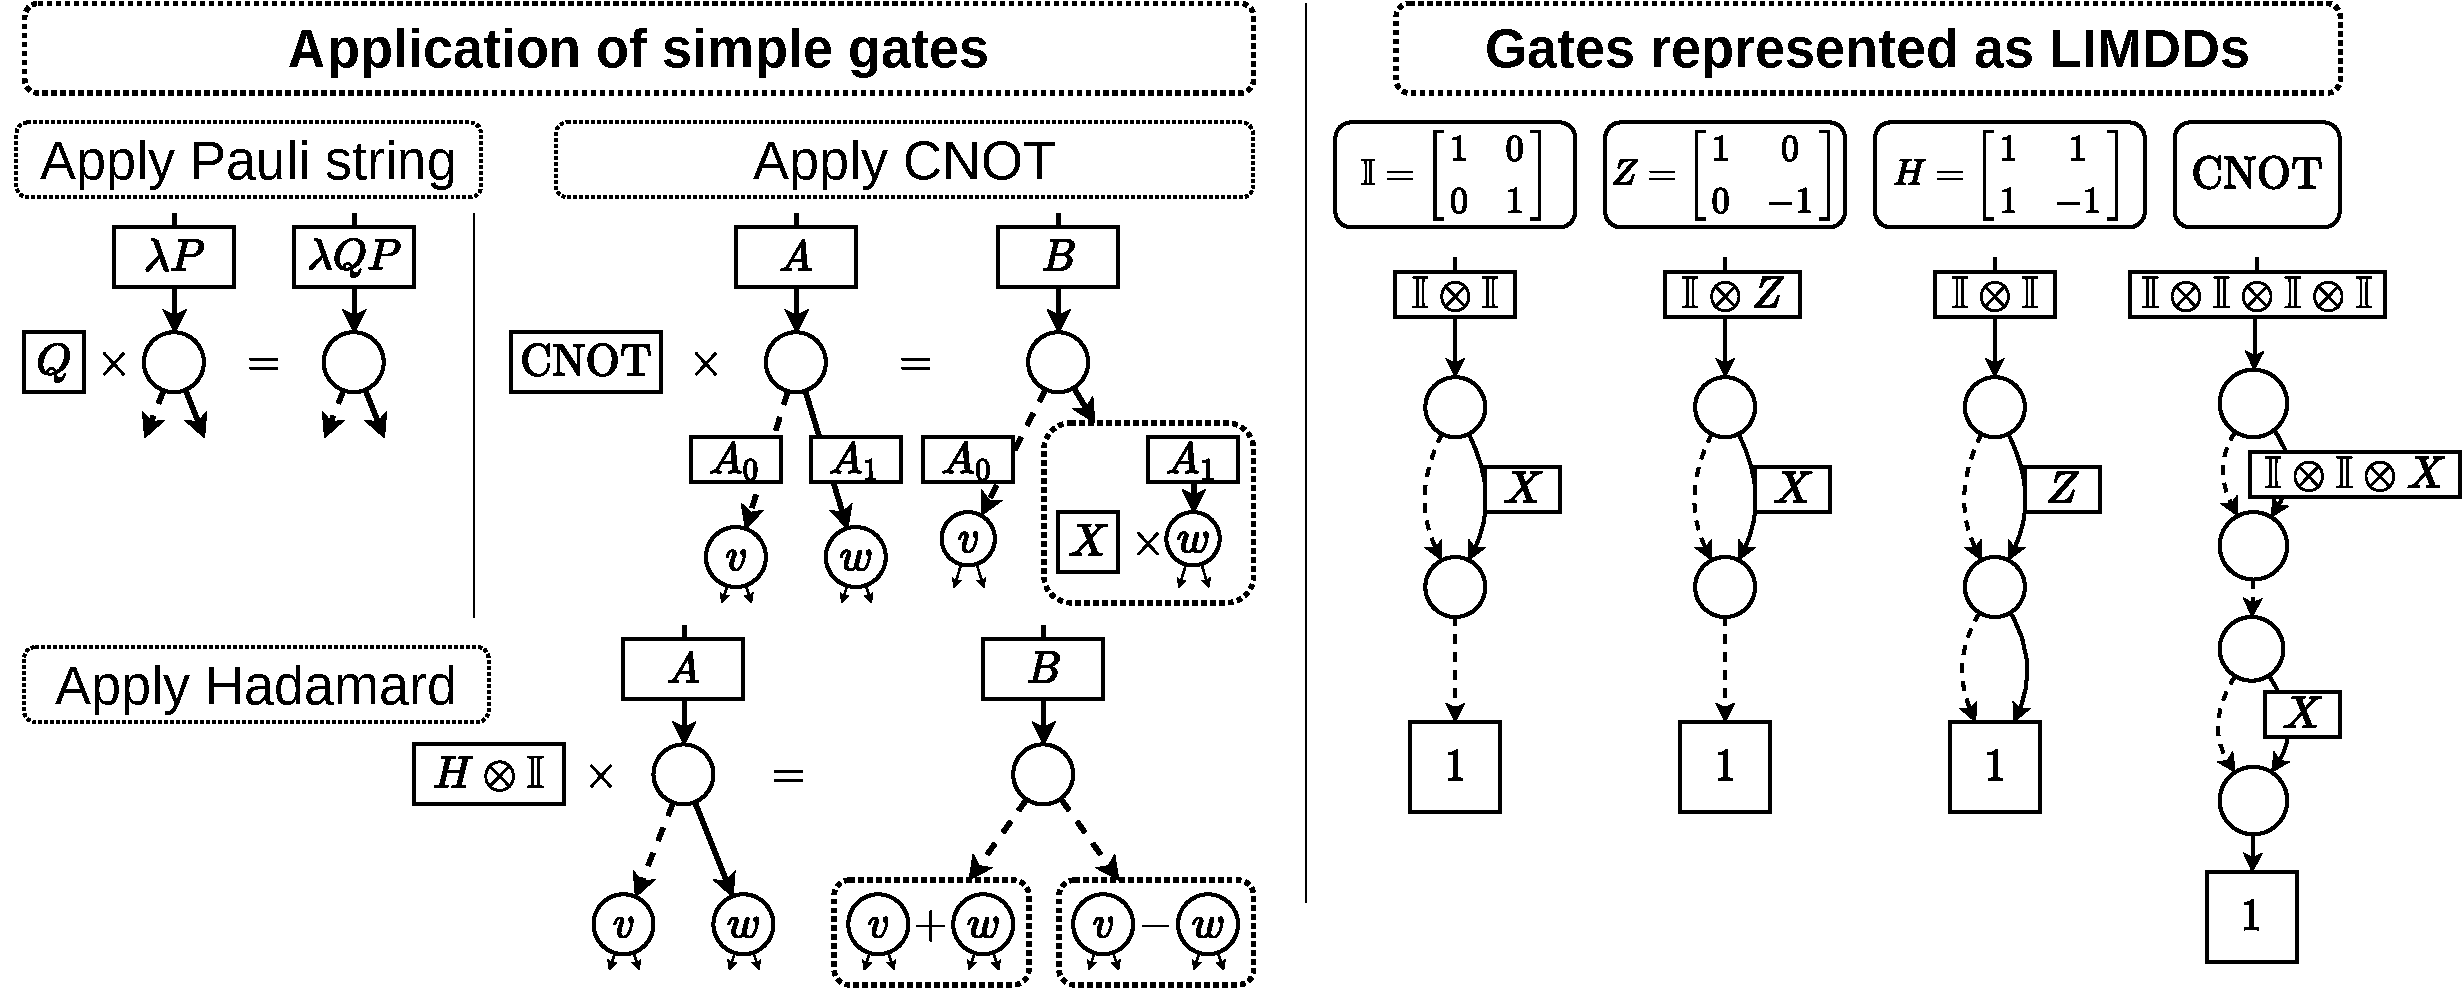
\includegraphics[width=\textwidth]{pics/gates-examples.pdf}
	\caption{\textbf{Left half}: illustration of applying several simple gates (some details are omitted).
		Leftmost: applying a Pauli string $Q$ to an edge entails only updating the label on that edge.
		Right: To apply a CNOT gate to the top qubit, apply $X\otimes \mathbb I^{\otimes n-2}$ to the right child; here this operation is represented inside a dotted box. The incoming edge's label changes from $A$ to $B=\text{CNOT}\cdot A\cdot\text{CNOT}$, which is guaranteed to be a Pauli string.
		Bottom: Applying a Hadamard gate on the top qubit is done by first making nodes representing $\ket{v}+\ket{w}$ and $\ket{v}-\ket{w}$, here shown in dotted boxes.
		\textbf{Right half}: Examples of four gates, represented as \limdds. Left: The identity gate $\mathbb I$ is represented by a \limdd of two levels. The first level indicates the row, and the second level indicates the column.
	Second from the right: the Hadamard gate; notice that the $Z$ label produces the $-1$ value in the matrix' bottom right entry.
	Rightmost: The CNOT gate. Since this gate is on $n=2$ qubits, it has $2n=4$ levels.
	Edges with label $\mathbb I$ are drawn without label; edges with label $0$ are not drawn.
	}
	\label{fig:gates-examples}
\end{figure}


%Here, we sketch algorithms for simulating quantum circuits using \limdds.
%In particular, \autoref{alg:apply-gate} shows how to apply a gate $\ket U$ to a state $\ket v$, where both  are represented as \limdds with root nodes $u$  and $v$.
%This recursive algorithm outputs (an edge to) a reduced \limdd $e$, representing $\ket{e}=U\ket{v}$.
%This edge is made on line \ref{algline:apply-gate-make-edge} with a call to \makeedge.
%This subroutine guarantees that the edge, and all nodes below it, satisfy all the reduction rules of \autoref{def:reduced-limdd}, making the result canonical.
%Consequently, all intermediate \limdds that are produced by the algorithm are reduced.

The procedure \textsc{ApplyGate} (\autoref{alg:apply-gate-limdd-limdd}) applies a gate $U$ to a state $\ket{\phi}$, represented by \limdds $e^u$ and $e^v$.
It outputs is a \limdd edge representing $U\ket{\phi}$.
%\autoref{alg:apply-gate} gives the procedure \textsc{ApplyGate} for updating a \limdd after applying an arbitrary gate $U$ to state $\ket \phi$ represented by \limdd edges $e^u$ and $e^v$.
%If we ignore the complexity\todo{we claim we can apply arbitrary gates, so we should do so or make clear immediately that we can.} 
%introduced by the labels on the edges $e^v$ and $e^U$\todo{$u$}, then the algorithm is quite straightforward:
It works as follows (see \autoref{fig:apply-gate} for an illustration).
Using the $\follow{x}{e}$ procedure, we write $\ket{\phi}$ and $U$ as
\begin{align}
	\ket{\phi} = & \ket{0}\ket{\phi_0}+\ket{1}\ket{\phi_1} \\
	U = & \ket{0}\bra{0}\otimes U_{00} + \ket{0}\bra{1}\otimes U_{01} + \ket{1}\bra{0}\otimes U_{10} + \ket{1}\bra{1}\otimes U_{11}
\end{align}
Then, on line \ref{algline:apply-gate-compute-term}, we compute each of the four terms $U_{rc}\ket{\phi_c}$ for row/column bits $r,c \in \{0,1\}$.
We do this by constructing four \limdds $f_{r,c}$ representing the states
$\ket{f_{r,c}}=U_{r,c}\ket{\phi_c}$, using four recursive calls to the \textsc{ApplyGate} algorithm.
Next, on lines \ref{algline:apply-gate-add-0} and \ref{algline:apply-gate-add-1}, the appropriate states are added, using \textsc{Add} (\autoref{alg:add-limdds}), producing \limdds $e_0$ and $e_1$ for the states $\ket{e_0}=U_{00}\ket{\phi_0}+U_{10}\ket{\phi_1}$ and for $\ket{e_1}=U_{01}\ket{\phi_0}+U_{11}\ket{\phi_1}$.
The base case of \textsc{ApplyGate} is the case where $n=0$, in which case both $e^u$ and $e^v$ are edges which point to the leaf, which means $U$ and $\ket{v}$ are simply scalars.

Here, too, we employ dynamic programming to prevent the algorithm from performing duplicate computations.
Namely, when we have computed the edge $e^{w}$, we store this result in the cache (line \ref{algline:apply-gate-store-cache}).
In subsequent calls, this result can be retrieved from the cache (on line \ref{algline:apply-gate-retrieve-cache}), recovering the result without performing the computation again.



\begin{algorithm}[htb!]
	\caption{Applies the gate $[e^u]$ to the state $\ket{e^v}$. Here $e^u$ and $e^v$ are \limdd edges. 
		The output is a \limdd edge $e^{w}$ satisfying $\ket{e}=[e^u]\ket{e^v}$. It assumes that
		$2\index(v) = \index(u)$.}
	\label{alg:apply-gate-limdd-limdd}
	\begin{algorithmic}[1]
		\Procedure{ApplyGate}{\Edge $\ledge[e^u] Au$, \Edge $\ledge[e^v] Bv$ \textbf{with} $A=\lambda_A P$, $B=\lambda_B Q$}
		\If{$A=0$ or $B=0$} \Return $0$
		\EndIf
		\If{$n=0$}  \Return $\ledge {AB}v$
%		\Else
        \EndIf
		\State $P^\prime, Q^\prime:=\rootlabel(\ledge Pu),\rootlabel(\ledge Qv)$ \Comment{Get canonical root labels}
		\If{$(\ledge {P^\prime}u,\ledge {Q^\prime} v)\in \textsc{Apply-cache}$}\Comment{Dynamic programming}
		\State \Return $\lambda_A \lambda_B \cdot \textsc{Apply-cache}[\ledge {P^\prime} u, \ledge {Q^\prime} v]$
			\label{algline:apply-gate-retrieve-cache}
		\EndIf
		%				\State edge $a_0:=\follow{0}{e^v}$
		%				\State edge $a_1:=\follow{1}{e^v}$
		\For{$r,c\in\{0,1\}$}
		%					\State edge $M_{r,c}:=\follow{rc}{e^U}$
		%				\EndFor
		%				\For{$r,c\in \{0,1\}$}
		\State \Edge $f_{r,c}:=\textsc{ApplyGate}(\follow{rc}{\ledge Qu},\follow{c}{\ledge Pv})$
			\label{algline:apply-gate-compute-term}
		\EndFor
		\State \Edge $e_0:=\textsc{Add}(f_{0,0}, f_{0,1})$
			\label{algline:apply-gate-add-0}
		\State \Edge $e_1:=\textsc{Add}(f_{1,0}, f_{1,1})$
			\label{algline:apply-gate-add-1}
		\State \Edge $e^{w}:=\makeedge(e_0,e_1)$
		\State $\textsc{Apply-cache}[\ledge {P^\prime}u, \ledge {Q^\prime}v]:=e^{w}$ \Comment{Store result in cache}
			\label{algline:apply-gate-store-cache}
		\State \Return $\lambda_A\lambda_B \cdot e^{w}$
			\label{algline:apply-gate-return}
%		\EndIf
		\EndProcedure
	\end{algorithmic}
\end{algorithm}


Specifically, we store a tuple $(P^\prime, u, Q^\prime, v)$ in the cache.
Here $P^\prime=\rootlabel(\ledge Pu)$ and $Q^\prime=\rootlabel(\ledge Qv)$ are canonically chosen LIMs.
By ``canonically chosen'', we mean that $Q^\prime\ket{v}=Q\ket{v}$, and that the procedure chooses the same LIM $Q^\prime$ for every $\ledge{Q''}{v}$ such that $Q^{\prime\prime}\ket{v}=Q\ket{v}$.
We do this so that, in a subsequent call to \textsc{ApplyGate} with inputs $(\ledge {\mu_AP^{\prime\prime}}u,\ledge {\mu_BQ^{\prime\prime}}v)$, we will find the correct result in the cache whenever $Q^{\prime\prime}\ket{v}=Q\ket{v}$, even if $Q^{\prime\prime}\ne Q$.

A specific choice for \rootlabel is the lexicographic minimum of all possible root labels, following a similar choice for making a canonical choice for the high edge label of a node in \autoref{sec:makeedge}.
In \autoref{alg:lexmin} in that section, we will give an $O(n^3)$-time algorithm for computing the lexicographically minimal root label.

Notice also that the scalars $\lambda_A,\lambda_B$ are not stored in the cache; they are factored out and multiplied as needed on lines \ref{algline:apply-gate-retrieve-cache} and \ref{algline:apply-gate-return}.
%To improve the performance of the cache, we ``factor out'' the scalars $\lambda_A$ and $\lambda_B$ before storing the result in the cache, storing only the tuple $(\ledge Qu,\ledge Pv)$.
%This allows a subsequent call to \textsc{ApplyGate} to retrieve the answer, even if, in that call, the LIMs on the input edges have different scalars.
Using similar reasoning, we also do not propagate these scalars into the recursive calls on line \ref{algline:apply-gate-compute-term}.
%We can further optimize the cache by observing that the even Pauli's in $A$
%(the label on the root edge of which represents the matrix) are 

%
\begin{figure}
	\centering
	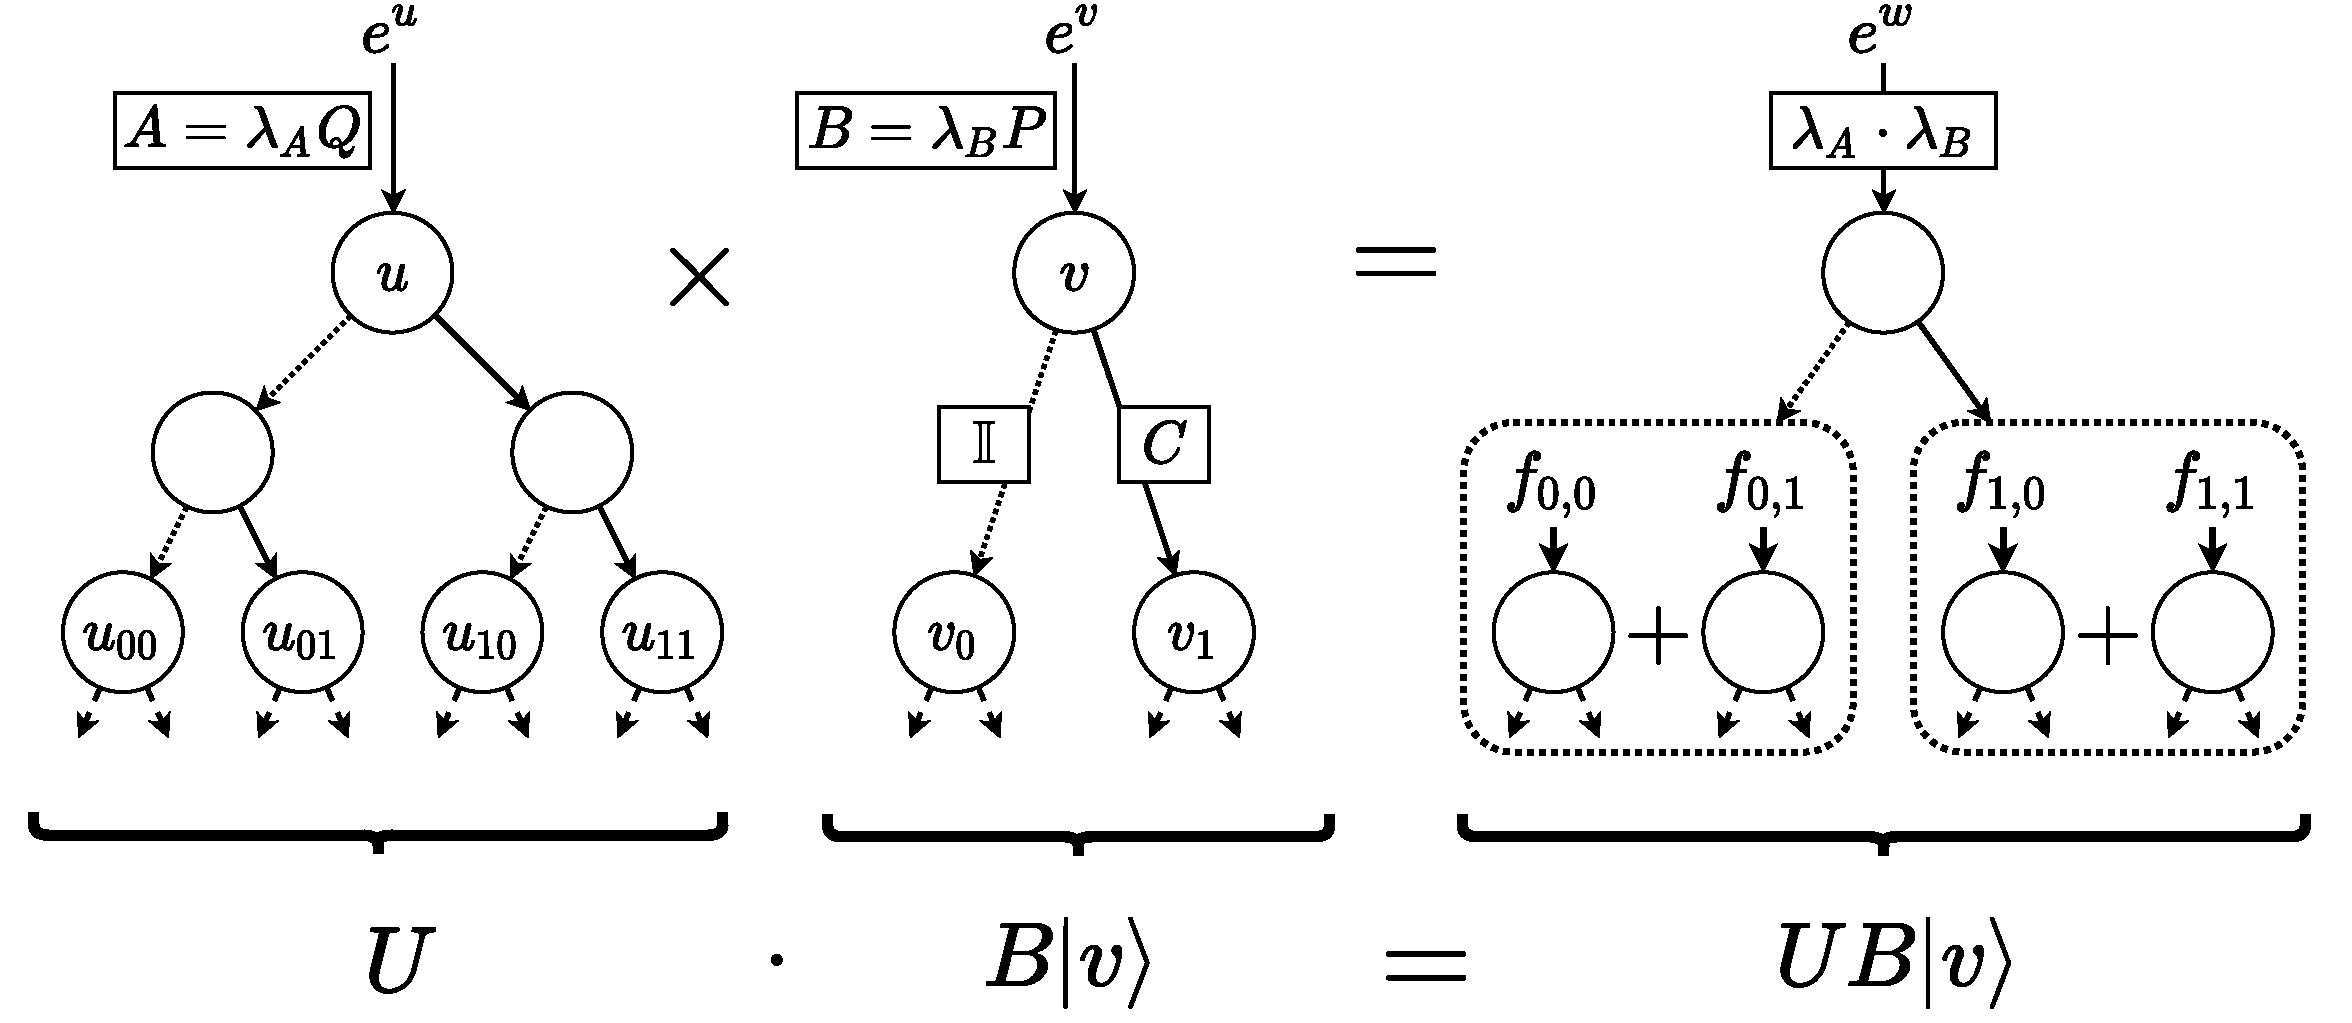
\includegraphics[width=.8\textwidth]{pics/apply-gate-2.pdf}
    \caption{An illustration of \textsc{ApplyGate} (\autoref{alg:apply-gate-limdd-limdd}), where matrix $U$ is applied to state $B\ket{v}$, both represented as Pauli-\limdds.
		The edges $f_{0,0}$, $f_{0,1}$, etc. are the edges made on line \ref{algline:apply-gate-compute-term}.
		The dotted box indicates that these states are added, using \textsc{Add} (\autoref{alg:add-limdds}) before they are passed to \makeedge.
%	For simplicity, this diagram assumes $P_n=\mathbb I$.
%	Notice that the LIM $P^\prime$ is ``propagated'' to the result. In the \textsc{ApplyGate} algorithm, this is accomplished using the $\follow{0}{Av}$ subroutine.
}
	\label{fig:apply-gate}
\end{figure}

The subroutine \textsc{Add} (\autoref{alg:add-limdds}) adds two quantum states, i.e., given two \limdds representing $\ket{e}$ and $\ket{f}$, it returns a \limdd representing $\ket e + \ket f$.
A natural way to implement this algorithm would have been to use the $\follow xe$ procedure to express the states as $\ket{e}=\ket{0}\ket{e_0} + \ket 1\ket{e_1}$ and $\ket{f}=\ket 0\ket{f_0} + \ket 1\ket{f_1}$, and then to call the algorithm recursively to construct the states $\ket{e_0}+\ket{f_0}$ and $\ket{e_1}+\ket{f_1}$.


\begin{algorithm}[b!]
	\begin{algorithmic}[1]
		\Procedure{Add}{\Edge $\ledge[e] Av$, \Edge $\ledge[f] Bw$
		 \textbf{with} $A=\lambda P$, $B=\mu Q$, $\index(v) = \index(w)$}
		\If{$n=0$}
			 \Return $\ledge {A+B}1$ \Comment{$A,B \in \mathbb C$}
		\EndIf
		\If{$v\not\beforeq w$} \Return $\textsc{Add}(f,e)$
		\label{algline:add-swap-for-cache}
		\EndIf
		\State $C:=\rootlabel(\ledge{A^{-1}B}{w})$
		\label{algline:add-factor-out-LIM}
		\If{$(v,\ledge Cw)\in \textsc{Add-cache}$} 
			\Return $A\cdot \textsc{Add-cache}[v,\ledge Cw]$ \Comment{Dynamic programming}
		\EndIf
		\State \Edge $a_0:=\textsc{Add}(\follow 0{\ledge{\mathbb I}v}, \follow 0{\ledge Cw})$
			\label{algline:add-0}
		\State \Edge $a_1:=\textsc{Add}(\follow 1{\ledge{\mathbb I}v}, \follow 1{\ledge Cw})$
			\label{algline:add-1}
		\State \Edge $a:=\makeedge(a_0,a_1)$ 
			\label{algline:add-makeedge}
		\State $\textsc{Add-cache}[v,\ledge Cw]:= a$
            \Comment{Store in dynamic programming cache}
		\State \Return $A\cdot a$
		\EndProcedure
	\end{algorithmic}
	\caption{Given two $n$-LIMDD edges $e,f$, constructs a new LIMDD edge $a$ with $\ket{a}=\ket{e}+\ket{f}$.
	}
	\label{alg:add-limdds}
\end{algorithm}

However, we implement the algorithm slightly differently in order to better take advantage of dynamic programming.
We remark that we are looking to construct the state $A\ket{v} + B\ket{w}$, and that this is equal to $A\cdot (\ket{v}+A^{-1}B\ket{w})$.
Therefore, letting $\ket{\psi}=A^{-1}B\ket{w}$, we use the $\follow x{\ledge{A^{-1}B}w}$ procedure to construct the states $\ket{\psi_0}$ and $\ket{\psi_1}$.
Then, we construct the states $\ket{a_0}=\ket{v_0}+\ket{\psi_0}$ and $\ket{a_1}=\ket{v_1}+\ket{\psi_1}$, on \autoref{algline:add-0} and \ref{algline:add-1}.
Lastly, we construct the state $\ket{a}=\ket{0}\ket{a_0}+\ket 1\ket{a_1}$, on line \ref{algline:add-makeedge}.
Returning the \limdd $A\cdot a$ yields the desired result:
\begin{align}
	A\ket{a} = & A(\ket{0}\ket{a_0}+\ket{1}\ket{a_1}) = A(\ket 0(\ket{v_0}+\ket{\psi_0}) + \ket 1(\ket{v_1}+\ket{\psi_1})) \\
	= & A(\ket{v}+\ket{\psi}) = A(\ket{v} + A^{-1}B\ket{w}) = A\ket{v} + B\ket{w}
\end{align}
We store a tuple $(v,w,C)$ in the cache, where $C=\rootlabel(\ledge {A^{-1}B}w)$ is a canonically chosen LIM such that $C\ket{w}=A^{-1}B\ket{w}$.
By ``canonically chosen'', we mean, again, that the procedure chooses the same $C$ for any input $\ledge Dw, \ledge Ew$ such that $D\ket{w}=E\ket{w}$. 

Finally, on line \ref{algline:add-swap-for-cache}, we use the total order on nodes $\beforeq$,
in order to prevent cache misses due to storing $v$ and $w$ in the wrong order.


%\alfons{It can be implemented in cubic time using the techniques described in } \autoref{sec:preliminaries}.\todo{this should be explained earlier, because it is used in the ApplyGate algorithm.}

%Let us see how implementing the algorithm this way improves the performance of the cache, relative to the straightforward way we have outlined.
%When, after input $(e,f)$, \textsc{Add} is subsequently called as $\textsc{Add}(e'=\ledge {D}{v'},f'=\ledge E{w'})$, then we achieve a cache hit whenever $v=v'$ and $A^{-1}B\ket{w}=D^{-1}E\ket{w'}$, whereas in the simpler implementation, we would have achieved a cache hit only when $A\ket{v}= D\ket{v'}$ and $B\ket{w}= E\ket{w'}$.
%Effectively, this means that we get a cache hit whenever $\ket{e}\simeq \ket{e'}$, instead of when $\ket{e}=\ket{e'}$.

\begin{wrapfigure}{r}{6cm}\vspace{-1em}
    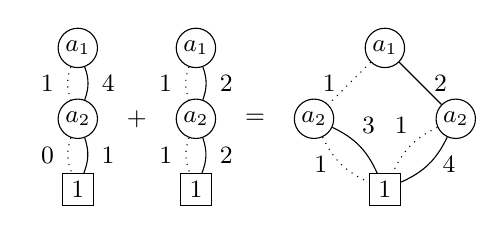
\begin{tikzpicture}[
        scale=0.3,
        every path/.style={>=latex},
        every node/.style={},
        inner sep=0pt,
        minimum size=0.5cm,
        line width=1pt,
        thin,
        font=\small
        ]

        % nodes

        % nodes
        \node[draw,circle] (a1) at ( 0,-0)     {$a_1$};
        \node[draw,circle] (a2) at (0,-3) {$a_2$};

        \node[draw,circle,rectangle,minimum size=0.4cm] (w1) at ( -0,-6) {$1$};

        % edges
        \draw[dotted,bend left=-20] (a1) edge  node[left] {$1$} (a2);
        \draw[bend left=20]        (a1) edge  node[right] {$4$} (a2);
        
        \draw[dotted,bend left=-20] (a2) edge node[left] {$0$} (w1);
        \draw[bend left=20]       (a2) edge  node[right] {$1$} (w1);


        \node[draw,circle] (a1) at (5,-0)     {$a_1$};
        \node[draw,circle] (a2) at (5,-3) {$a_2$};

        \node[draw,circle,rectangle,minimum size=0.4cm] (w1) at ( 5,-6) {$1$};

        % edges
        \draw[dotted,bend left=-20] (a1) edge  node[left] {$1$} (a2);
        \draw[bend left=20]        (a1) edge  node[right] {$2$} (a2);
        
        \draw[dotted,bend left=-20] (a2) edge node[left] {$1$} (w1);
        \draw[bend left=20]       (a2) edge  node[right] {$2$} (w1);


        \node[draw,circle] (a1p) at ( 13,-0)     {$a_1$};
        \node[draw,circle] (a20) at ( 10,-3) {$a_2$};
        \node[draw,circle] (a21) at ( 16,-3) {$a_2$};

        \node[draw,circle,rectangle,minimum size=0.4cm] (w1) at ( 13,-6) {$1$};

        % edges
        \draw[dotted] (a1p) edge  node[left] {1} (a20);
        \draw[]     (a1p) edge  node[right] {2} (a21);
        
        \draw[dotted,bend left =-20] (a20) edge  node[left] {1} (w1);
        \draw[      ,bend left = 20]       (a20) edge  node[above right, xshift=-4pt] {3} (w1);
        
        \draw[dotted,bend left =-20] (a21) edge node[above left, xshift=4pt] {1} (w1);
        \draw[      ,bend left = 20]       (a21) edge  node[right] {4} (w1);
        
        
        \node[] (a2) at (2.5,-3) {$+$};
        \node[] (a2) at (7.5,-3) {$=$};
        
    \end{tikzpicture}
    \caption{Adding two states \vect{0,1,0,4} and \vect{1,2,2,4} as \qmdds can cause an exponentially larger result \qmdd  \vect{1,3,2,8} due to the loss of common factors.}
    \label{fig:explosion}
\end{wrapfigure}

The worst-case running time of \textsc{Add} is $\oh(n^32^n)$, if $n$ is the number of qubits.
The resulting \limdd can be exponential in the input sizes (bounded by $2^n$),
and \textsc{Add} calls \makeedge has runtime $\oh(n^3)$.
This exponential result happens already for \qmdds because the addition might remove any common factors that can be factored out as illustrated in \autoref{fig:explosion}.
%every recursive call effects a cache miss, so that in total $\oh(2^n)$ recursive calls are made.
This exponential-time worst-case behavior  for \qmdds (and related DDs)
 was identified \cite[Table 2]{fargier2014knowledge} and is inherited by \limdds.
However, the \textsc{Add} algorithm is polynomial-time when $v=w$ and $v$ is a stabilizer state (\autoref{thm:only-linear-recursive-add-calls-general})
% Note however, that the corresponding \add would already be exponential


\subsection{The \makeedge subroutine}
\label{sec:makeedge}


To construct new nodes and edges, our algorithms use the \makeedge subroutine as discussed above.
\makeedge produces reduced parent nodes for reduced children, so that the \limdd representation becomes canonical; an important property for efficient manipulation algorithms and analysis techniques. 
Here we give the algorithm for \makeedge and show that it runs in time $O(n^3)$ (assuming the input nodes are reduced).

%\todo[inline]{I think \autoref{sec:makeedge-basic-reduction} makes nodes reduced, not semi-reduced? Let me double-check -LV}
We call a \limdd node \concept{semi-reduced}, if it satisfies the
{low factoring, low precedence, zero edge and merge rules} of \autoref{def:reduced-limdd}, i.e., if it satisfies all reduction rules except possibly high determinism.
Semi-reduction is easy to enforce, as shown in \autoref{sec:makeedge-basic-reduction}.
The bulk of this section discusses how to obtain a canonical LIM on the high edge
to realize high determinism.
We achieve this  in \autoref{sec:choose-canonical-isomorphism-pauli} by selecting a lexicographically minimum LIM from all the candidates.
The problem of find all candidates efficiently is reduced to finding all stabilizers of a state $\ket v$,
i.e., the set of all LIMs $A$ such that $A \ket v = \ket v$, efficiently represented as a set of generators (see also \autoref{sec:preliminaries}).
In \autoref{sec:pauli-isomorphism-detection}, we show how to compute these stabilizers in the bottom-up fashion typical for decision diagrams.


%\begin{lemma}
%    For any Tower \limdd, the procedure  \textsc{Add} takes $\oh(n^4)$ time.   
%\end{lemma}
%\begin{proof}
%    Let $\ledge {B_n}{v_n}$ be the root edge of a Tower  with nodes $v_n, \dots v_1, v_0 = \leaf$ and edges
%    $\Low = \High = \set{ (v_i, v_{i-1}) \mid i \in \set{0, \dots, n} }$ with labels
%    $\lbl(\high{v_i}) = B_i$, $\lbl(\low{v_i}) = \id$.   
%    Using induction, we find that in the base case $n=0$, $B_n$ is a scalar so the resulting 
%\end{proof}


\subsubsection{Basic reduction in MakeEdge}
\label{sec:makeedge-basic-reduction}

%\todo[inline]{Question 2: Why is it called a root edge, when most nodes are not the root? If I look in \autoref{def:limdd}, then the root node is the distinguished top node. Maybe we should call it, ``incoming edge''? -LV One way to view it is that our algorithms create many \limdds (some overlapping). Because it is all sequential, usually only one or two exist at the same time.}

\autoref{alg:make-edge} gives the \makeedge subroutine that now
constructs canonical nodes through reduction, yielding a new root edge (whose LIM label is not necessarily canonical).
It takes as input two edges $e_0$ and $e_1$, pointing to already reduced nodes, and outputs an edge $e$, pointing to a reduced node $v$,
such that $\ket{e}=\ket{0}\ket{e_0}+\ket{1}\ket{e_1}$.
The reduction proceeds as follows.
\begin{itemize}
    \item 
First it ensures low precedence, switching $e_0$ and $e_1$ if necessary at
\autoref{l:swap}. This is also done if $e_0$'s label $A$ is $0$ to allow for low factoring (avoiding divide by zero).
    \item 
Low factoring, i.e., dividing
out the LIM $A$, placing it on the root node,
        is visualized in \autoref{fig:reduced1} for the cases $e_1 = 0 / e_1\neq 0$,
and done in the algorithm at \autoref{l:low1},\ref{l:low2} / \ref{l:low3},\ref{l:low4}.
\item 
The zero edges rule is enforced in the $B=0$ branch by taking $v_1 := v_0$.
\item 
The canonical high label $\highlim$ is computed by \textsc{GetLabels},
    discussed below, for low factored node $\lnode[w] {\id}{v_0}{\hat A}{v_1}$.
    It satisfies the high determinism rule of \autoref{def:reduced-limdd} with $\highlabel(w)= \highlim$
    as shown in the next section with \autoref{cor:highlabel}.
\item
Finally, we merge nodes by creating an entry $(v_0,\highlim,v_1)$ in 
a \concept{unique table}~\cite{brace1990efficient} at \autoref{algline:find-v-in-unique}. 
\end{itemize}

All steps except for \textsc{GetLabels} have complexity $O(1)$ or $O(n)$ (for checking low precedence, we use nodes' order in the unique table).
\textsc{GetLabels} has a runtime $O(n^3)$ as we show in \autoref{sec:choose-canonical-isomorphism-pauli}, yielding an overall complexity $O(n^3)$.
%\todo{I think the reducedness of the children is no longer required, provided we phrase the resulting reduction as dependent on the reducedness of these inputs.}

\begin{algorithm}
	\begin{algorithmic}[1]
        \Procedure{MakeEdge}{\Edge $\ledge[e_0]{A}{v_0}$, \Edge $\ledge[e_1]{B}{v_1}$ 
                        , where $v_0, v_1$ reduced, \textbf{with} $A \neq 0$ \textbf{or} $B \neq 0$}
%    		\State \textbf{assert} $\index(v_0) = \index(v_1)$
%    		\State $n := \index(v_0)$
            \If{$v_0\not\beforeq v_1$ \textbf{or} $A=0$} \Comment{Enforce \textbf{low precedence} and enable \textbf{factoring}}
                \State \Return\label{l:swap}
                        $(X \otimes \unit_2^{\otimes n})\cdot \text{MakeEdge}(e_1, e_0)$
                        %\ledge{B}{v_1},\ledge{A}{v_0})$
%                \todo[inline]{Tim: do we already have notation for multiplying an edge with a LIM?} %Alfons: Yes. See table
			\EndIf
            %
            %
%            \Comment{Enforce \textbf{low factoring}}
%            \State $w_0 := v_0$
            \If{$B = 0$}
            \State $v_1 := v_0$     \Comment{Enforce  \textbf{zero edges}}
            \State $v := \lnode{\unit_2^{\otimes n}}{v_0}{0}{v_0}$\label{l:low1}
            \Comment{Enforce \textbf{low factoring}}
%            \State $\highlim := 0$
%            \State $w_1 := v_0$
%			\Comment{Enforce \textbf{}}
            %
            %
            \State $\rootlim := \unit_2 \otimes A$   \Comment{$\rootlim \ket v = \ket 0 \otimes 
                                        A \ket{v_0} + \ket 1 \otimes  B \ket{v_1}$}\label{l:low2}
            \Else
            %
            %
            \State $\hat A := A^{-1}B$ \Comment{Enforce \textbf{low factoring}}\label{l:low3}
            \State $\highlim, \rootlim:=\textsc{GetLabels}(\hat A,v_0,v_1)$
            \label{algline:makeedge-get-labels}
            \Comment{Enforce \textbf{high determinism}}
            \State $v := \lnode{\unit_2^{\otimes n}}{v_0}{\highlim}{v_1}$ 
             \Comment{$\rootlim \ket v = \ket 0 \otimes 
                                         \ket{v_0} + \ket 1 \otimes A^{-1} B \ket{v_1}$}
                \label{l:low4}
            \State $\rootlim := (\id[2] \otimes A) \rootlim $ 
             \Comment{$(\id[2] \otimes A)\rootlim \ket v = \ket 0 \otimes  A \ket{v_0} + \ket 1 \otimes  B \ket{v_1}$}
            \EndIf
%			\State node $v := Node(v_0,v_1,\hat A)$ representing $\ket{0}\ket{v_0}+\ket{1}\hat A\ket{v_1}$
			\State $v^r:=$ Find or create unique table entry $\unique[v] = (v_0, \highlim, v_1)$       
			\label{algline:find-v-in-unique}
            \Comment{Enforce \textbf{merge}}
            \State \Return $\ledge{\rootlim}{v^r}$
		\EndProcedure
	\end{algorithmic}
	\caption{
        Algorithm \makeedge takes two root edges to (already reduced) nodes $v_0,v_1$, the children of a new node, and returns a reduced node with root edge.
	It assumes that %the children have the same qubit-index, i.e., 
	$\index(v_0) = \index(v_1) = n$.
%	For sake of simplicity, this algorithm does not enforce the root edge determinism rule, nor the zero edges rule.
	We indicate which lines of code are responsible for which reduction rule in \autoref{def:reduced-limdd}.
}
	\label{alg:make-edge}
\end{algorithm}

\begin{figure}
    % CASE: different children nodes
\tikz[->,>=stealth',shorten >=1pt,auto,node distance=1.5cm,
        thick, state/.style={circle,draw,inner sep=0pt,minimum size=18pt}]{
    %\node[state, above = 2cm of 1, xshift=3.3cm] (top) {};

    \node[state] (2) {$w$};
    \node[state] (1a) [below = 1cm of 2, xshift=1.3cm] {$v_0$};
    \node[right = 0.25cm of 1a] () {$\beforeq$};
    \node[state] (1b) [below = 1cm of 2, xshift=2.8cm] {$v_1$};
    \node[above = 0.5cm of 2,xshift=1.95cm,fill=black] (x)  {};
    \path[]
    (x) edge[bend left=-20]    node[above right,pos=.8] {} (2)
    (2) edge[e0] node[pos=.5,left] {$\id[2]^{\otimes n}$} (1a)
    (2) edge[e1] node[pos=.15,right, xshift = .5cm] {$\lambda P$} (1b)
    ;
    
    \node[state, right = 3.3cm of 2] (4) {$v^{\textnormal{r}}$};
%    \node[above = 0.5cm of 4] (x)  {};
    \path[]
    (x) edge[bend left=20]     node[pos=.9] {
        $\rootlim = \left(\lambda X\otimes P\right)^{x} \cdot
        \left(Z^s \otimes \left(\gmax_0\right)^{-1}\right)$
        } (4)
    (4) edge[e0] node[pos=.3,above left] {$\id[2]^{\otimes n}$} (1a)
    (4) edge[e1] node[pos=.3,below right] {
%    \begin{minipage}{5cm}
        $\highlim = %(-1)^s \cdot \lambda^{(-1)^x} \cdot \gmax_0 \cdot P \cdot \gmax_1 = 
%                    \displaystyle \min_{i,s,x \in \{0, 1\},g_i \in \Aut(v_i)}(\textnormal{\sc EligibleHigh}_{x,s,g_0,g_1})
%			\displaystyle \min_{i,x\in \{0,1\},g_{0/1}\in \Stab(v_{0/1})}
			(-1)^s\lambda^{(-1)^x}g_0Pg_1
        $
%    \end{minipage}
    } (1b)
    (2) --  node[yshift=.1cm] {$\rightsquigarrow$} (4)
    (1a)  edge[loop left, dashed] node[left]{$g_0\in\Aut(v_0)$} (1a)
    (1b)  edge[loop right, dashed] node[right]{$\Aut(v_1) \ni g_1$} (1b)
    ;
    }
    %
    %
    %
    \vspace{1mm}
    \newline
    \centering
    Choose $s,x\in \{0,1\},g_0\in \Stab(v_0),g_1\in \Stab(v_1)$ s.t. $\highlim$ is minimal and $x=0$ if $v_0=v_1$.
    %$
%    \highlim=\displaystyle \min_{i,x\in \{0,1\},g_{0/1}\in \Stab(v_{0/1})}(-1)^s\lambda^{(-1)^x}g_0Pg_1
%    \textnormal{\sc EligibleHigh}_{x,s,g_0,g_1}  \defn
%        \set{(-1)^s \cdot \lambda^{(-1)^x} \cdot g_0 \cdot P \cdot g_1 ~\Big|~ %g_i \in \Aut(v_i),
        %\quad , \quad 
%         x \neq 1 \text{ if } v_0 \neq v_1 }
%     $
    %
	\caption{
        Illustration of finding a canonical high label for a semi-reduced node $w$,
        yielding a reduced node $v^{\text{r}}$.
%         which satisfies Low Precedence ($v_0 \beforeq v_1$) and Low Factoring (low edge is $\id[2]^{\otimes n}$).
The chosen high label is the minimal element from the set of eligible high labels
based on stabilizers $g_0,g_1$ of $v_0,v_1$ (drawn as self loops).
The minimal element holds a factor $\lambda^{(-1)^x}$ for some $x \in \{0, 1\}$.
There are two cases: if $v_0 \neq v_1$ or $x=0$, then the factor is $\lambda$ and the root edge should be adjusted with an $\id[2]$ or $Z$ on the root qubit.
The other case, $x=1$, leads to an additional multiplication with an $X$ on the root qubit.
%The result is a node $v^{\textnormal{reduced}}$ which satisfies Low Precedence, Low Factoring and High Determinism.
}
	\label{fig:reduced}
\end{figure}


%\todo[inline]{first explain the data structure \automorphismgenerators, i.e. that it can be thought of as spanning a vector space, and then give the algorithm}


%Data structure {\sc SystemOfPauliEquations}
%is a list of equations of the form $\lambda P (\alpha \ket{\phi}) = \beta \ket{\psi}$.
%Has a method {\sc 


\subsubsection{Choosing a canonical high-edge label}
\label{sec:choose-canonical-isomorphism-pauli}

%The \textsc{MakeEdge} procedure enforces that all reduction rules are satisfied, one by one.
%For all reduction rules except for a canonical high-label choice this is straightforward, e.g. for Low Precedence, if the right child $\succ$ the left child, then swap them and apply the appropriate Pauli at the root label.

On line \ref{algline:makeedge-get-labels}, the \makeedge algorithm finds a canonical label $\highlim$ for the high edge of node $v$ with a call to \textsc{GetLabels}.
%The semi-reduced node  \lnode[w]{\unit_2^{\otimes n}}{v_0}{\hat A}{v_1} with $v_0 \neq v_1$ created in
%\makeedge is passed to \textsc{GetLabels} to obtain a canonical
%representative \lnode[v^{\text{r}}]{\unit_2^{\otimes n}}{v_0}{\highlim}{v_1}
% (with `r' for reduced) and a root edge $\ledge[e] {\rootlim}{v^{\text{r}}}$ such that
% $\ket e = \ket w$.
It does so by taking the lexicographically minimal candidate for \highlim, see \autoref{sec:preliminaries}.
We now first characterize all eligible labels \highlim, by reducing the problem to finding stabilizer subgroups of the children nodes $v_0,v_1$ (see \autoref{sec:preliminaries}), denoted as $\Stab(v_0)$ and $\Stab(v_1)$.
Then, we show that \textsc{GetLabels} (\autoref{alg:find-canonical-edges}) correctly finds the lexicographically minimal eligible LIM (and corresponding root label), and runs in time $O(n^3)$ where $n$ is the number of qubits.

\autoref{fig:reduced} illustrates this process.
It shows the status of the \makeedge algorithm on line \ref{algline:makeedge-get-labels}, when it has enough information to construct the semi-reduced node $\lnode[w]{\id^{\otimes n}}{v_0}{\hat A}{v_1}$, with $\hat A=\lambda P$ on its high edge, shown on the left.
The set of eligible high labels is shown, and the lexicographically minimal is chosen as $\highlim$, yielding a new node $v^r$ (with `r' for `reduced').
This set of labels is decomposed into a choice of $v_0,v_1$ stabilizer $g_0, g_1$ and a choice for the most significant
\Pauli operator on the root LIM $X^x Z^s$.
\autoref{thm:eligible-isomorphisms-pauli} shows that this captures all possible high edges.



%\begin{lemma}
%    \label{lemma:isomorphic-nodes-have-same-high-label-scalar}
%    Let $\lambda, \mu \in \mathbb{C}$ and let $A, B$ be Pauli strings of length $n$.
%    Furthermore, let $v$ be the $n$-qubit root node of a reduced Pauli-\limdd.
%    If $\ket{\lambda A} \psim \ket{\mu B}$, then $\lambda = \mu$.
%\end{lemma}
%\begin{proof}
%    By induction...still to do
%\end{proof}



%\todo[inline]{Tim: maybe we should instead of Automorphism group, talk about Stabilizer group. Potential disadvantage is that readers who skim the work incorrectly assume that this is about groups which characterize stabilizer states, i.e. the group is maximal, making our algorithms look like a new (and stupid) way to simulate stabilizer states}

\begin{theorem}
    [Eligible high-edge labels]
	\label{thm:eligible-isomorphisms-pauli}
    Let $\lnode[w]{\id[2]^{\otimes n}}{v_0}{\lambda P}{v_1}$ be a semi-reduced $n$-qubit node
    in a Pauli-\limdd, where $v_0, v_1$ are reduced, $P$ is a Pauli string and $\lambda \neq 0$.
    For all nodes $v = \lnode[v]{\id[2]^{\otimes n}}{v_0}{\highlim}{v_1}$, it holds that $\ket{w} \simeq \ket{v}$  if and only if 
    %\todo[inline]{Tim: I just realised that the statement should be: for all semi-reduced $w$: $\ket{w} \simeq \ket{v}$ if and only if $w$ has children $v_0$ and $v_1$, and the eligible high labels are of the form \dots. Should redo}
    \begin{equation}
        \label{eq:eligible-high-label}
    \highlim = (-1)^s \cdot \lambda^{(-1)^x} g_0 P g_1
    \end{equation}
        for some $g_0 \in \Aut(v_0), g_1 \in \Aut(v_1), s,x\in \{0, 1\}$ and
        $x=0$ if $v_0 \neq v_1$.
    An isomorphism mapping $\ket{w}$ to $\ket{v}$ is 
    \begin{equation}
        \label{eq:root-label-eligible-high-label}
        \rootlim = (X \otimes \lambda P)^{x} \cdot (Z^s \otimes (g_0)^{-1}).
    \end{equation}
\end{theorem}
\begin{proof}
    It is straightforward to verify that the isomorphism $\rootlim$ in eq.~\eqref{eq:root-label-eligible-high-label} indeed maps $\ket{w}$ to $\ket{v}$ (as $x = 1$ implies $v_0 = v_1$), which shows that $\ket{w} \simeq \ket{v}$.
    For the converse direction, suppose there exists an $n$-qubit Pauli LIM $C$ such that $C\ket{w} = \ket{v}$, i.e.
    \begin{equation}
        \label{eq:eligible-proof}
        C
        \left(\ket{0}\otimes \ket{v_0} + \lambda \ket{1} \otimes P \ket{v_1}\right)
        =
        \ket{0}\otimes \ket{v_0} + \ket{1} \otimes \highlim \ket{v_1}
        .
    \end{equation}
    We show that if $\highlim$ satisfies eq.~\eqref{eq:eligible-proof}, then it has a decomposition as in eq.~\eqref{eq:eligible-high-label}.
    \def\brest{C_{\textnormal{rest}}}
    \def\qtop{Q_{\textnormal{top}}}
    We write $C = \qtop \otimes \brest$ where $\qtop$ is a single-qubit Pauli operator and $\brest$ is an $(n-1)$-qubit Pauli LIM (or a complex number $\neq 0$ if $n=1$).
    We treat the two cases $\qtop \in \{\unit_2, Z\}$ and $\qtop \in \{X, Y\}$ separately:

    \textbf{Case $\boldsymbol{\unit_2, Z}$.} Then $\qtop = \begin{smallmat} 1& 0\\0 & (-1)^y\end{smallmat}$ for $y \in \{0, 1\}$.
        In this case, eq.~\eqref{eq:eligible-proof} implies $\brest \in \Aut(\ket{v_0})$ and $(-1)^y\lambda \brest P \ket{v_1} = \highlim \ket{v_1}$, or, equivalently, $(-1)^{-y} \lambda^{-1} P^{-1} \brest^{-1} \highlim \in \Aut(v_1)$.
        Hence, by choosing $s = y$ and $x = 0$, we compute
        \[
            (-1)^y \lambda^{(-1)^0} \underbrace{\brest}_{\in \Aut(v_0)} P \underbrace{(-1)^{-y} \lambda^{-1} P^{-1} \brest^{-1} \highlim}_{\in \Aut(v_1)}
            =
            \frac{(-1)^{y} \lambda^{(-1)^0}}{ (-1)^y \lambda} \highlim
            =
            \highlim
        \]
    \textbf{Case $\boldsymbol{X, Y}$.} Write $\qtop = \begin{pmatrix}0& z^{-1}\\ z&0\end{pmatrix}$ where $z \in \{1, i\}$. Now, eq.~\eqref{eq:eligible-proof} implies
		\begin{equation}
		    \label{eq:z}
            z \brest \ket{v_0} = \highlim \ket{v_1}
		\qquad\textnormal{and}\qquad
            z^{-1} \lambda \brest P \ket{v_1} = \ket{v_0}.
		\end{equation}
From eq.~\eqref{eq:z}, we first note that $\ket{v_0}$ and $\ket{v_1}$ are isomorphic, so by Corollary~\ref{cor:node-canonicity-strong}, we have $v_0 = v_1$.
    Consequently, we find from eq.~\eqref{eq:z} that $z^{-1}\brest^{-1} \highlim \in \Aut(v_0)$ and $z^{-1}\lambda \brest P \in \Aut(v_1)$.
    Now choose $x=1$ and choose $s$ such that $(-1)^s \cdot z^{-2} \brest^{-1} \highlim \brest = \highlim$ (recall that Pauli LIMs either commute or anticommute, so $\highlim\brest = \pm \brest \highlim$).
    This yields:
    \[
        (-1)^s \lambda^{-1} \cdot \underbrace{z^{-1}\brest^{-1} \highlim}_{\in \Aut(v_0)} \cdot P \cdot \underbrace{z^{-1} \lambda P \brest}_{\in \Aut(v_1)}
        =
        \lambda^{-1} \cdot \lambda \cdot
        (-1)^s 
        z^{-2} \cdot \left(\brest^{-1} \highlim \brest \right)
        =
        \highlim
    \]
    where we used the fact that $P^2 = \id[2]^{\otimes (n-1)}$ because $P$ is a Pauli string.
\end{proof}

%Next, we define a lexicographic ordering on LIMs:

\begin{corollary}\label{cor:highlabel}
As a corollary of \autoref{thm:eligible-isomorphisms-pauli}, we find that taking, as in \autoref{fig:reduced},
\[
\highlabel(\lnode[v] {\id}{v_0}{\lambda P}{v_1}) = \displaystyle \min_{\hspace{-3mm} i,s,x \in \{0, 1\},g_i \in \Aut(v_i)}(\set{(-1)^s \cdot \lambda^{(-1)^x} \cdot g_0 \cdot P \cdot g_1 ~\Big|~ 
         x \neq 1 \text{ if } v_0 \neq v_1 })
\]
yields a proper implementation of \highlabel as required by \autoref{def:reduced-limdd},
because it considers all possible \highlim such that
$\ket v \simeq_{\Pauli} \ket{0}\ket{v_0}+\ket{1}\otimes \highlabel(v)\ket{v_1}$.
\end{corollary}



% todo the procedure which chooses the lexmin element, not which constructs the isomorphism; this causes confusion

%, with high edge label $\lambda P$ and children $v_0, v_1$ as input, computes the minimal eligible high edge label and the root edge label that preserves the represented quantum state.
A naive implementation for \textsc{GetLabels} would follow the possible decompositions of eligible LIMs (see eq.~\eqref{eq:eligible-high-label}) and attempt to make this LIM smaller by greedy multiplication, first  with stabilizers of
$g_0 \in \Aut(v_0)$, and then with stabilizers $g_1\in \Aut(v_1)$.
To see why this does not work, consider the following example:
the high edge label is $Z$ and the stabilizer subgroups $\Aut(v_0) = \langle X\rangle$ and $\Aut(v_1) = \langle Y \rangle$.
Then the naive algorithm would terminate and return $Z$ because $X, Y> Z$, which is incorrect since the high-edge label $X \cdot Z \cdot Y = -i \id[2]$ is smaller than $Z$.

\begin{algorithm}
	\caption{
		Algorithm for finding the LIMs $\highlim$ and $\rootlim$ required by \makeedge.
		The LIM $\highlim$ is chosen canonically as the lexicographically smallest LIM in 
		the set characterized in \autoref{thm:eligible-isomorphisms-pauli}.
		It runs in $O(n^3)$-time (with $n$ the number of qubits),
		provided $\getautomorphisms$ has been computed for the children $v_0, v_1$.
		\label{alg:find-canonical-edges}
	}
	\begin{algorithmic}[1]
		\Procedure{GetLabels}{PauliLim $\lambda P \neq 0$ (current high label), reduced children nodes $v_0, v_1$}
		\Statex \textbf{Output}: canonical high label $\highlim$ and root label $\rootlim$
		\State $G_0, G_1 := \getautomorphisms(v_0), \getautomorphisms(v_1)$
		\State $(g_0, g_1) := \textsc{ArgLexMin}(G_0, G_1, \lambda P)$
%		\label{line:getlabels-min}
		\label{line:getlabels-argmin}
%		\State $A := \lambda P \cdot g_0 \cdot g_1$
%		\Comment $A = \textsc{LexMin}(G_0, G_1, \lambda P)$
		%        \State \textbf{if} $P$ and $g_0$ commute \textbf{then} $t:=0$ \textbf{else} $t:=1$
		%        \label{line:sign-error}
		%        \Comment $A =  (-1)^t \cdot g_0 \cdot \lambda P \cdot g_1$
		%
		\If{$v_0=v_1$}
		\label{algline:getlabels-start-minimizing}
		\State $(x,s):=\displaystyle\argmin_{(x,s)\in\{0,1\}^2}(-1)^s\lambda^{(-1)^x}g_0Pg_1$
		\Else
		\State $x:=0$
		\State $s:=\displaystyle \argmin_{s\in \{0,1\}} (-1)^s\lambda g_0Pg_1$
		\label{line:minimized-lim} 
		\EndIf
		%        \State $x := 0$
		%        \If {$v_0 = v_1$}  x  := $\displaystyle\argmin_{ 
		%             x\in \set{0, 1}}  
		%        \set{ (-1)^t \cdot \lambda^{(-1)^x} \cdot g_0 \cdot P \cdot g_1}$
		%        \Comment see \autoref{thm:eligible-isomorphisms-pauli}
		%        \EndIf
		%        \State $s:= \displaystyle\argmin_{s\in \set{0,1}}\set{(-1)^s\cdot (-1)^t \lambda^{(-1)^x} \cdot g_0 \cdot  P  \cdot g_1} $
		\State $\highlim := (-1)^s \cdot \lambda^{(-1)^x} \cdot g_0 \cdot P \cdot g_1$
		\State $\rootlim := (X \otimes \lambda P)^{x} \cdot (Z^s \otimes (g_0)^{-1})$
		%
		\State \Return $(\highlim, \rootlim)$
		\EndProcedure
	\end{algorithmic}
\end{algorithm}

To overcome this, we consider the group closure of \emph{both} $\Aut(v_0)$ \emph{and} $\Aut(v_1)$.
See \autoref{alg:find-canonical-edges} for the $O(n^3)$-algorithm for \textsc{GetLabels}, which proceeds in two steps.
In the first step (\autoref{line:getlabels-argmin}), we use the subroutine \textsc{ArgLexMin} for finding the minimal Pauli LIM $A$ such that $A = \lambda P \cdot g_0 \cdot g_1$ for $g_0\in \Aut(v_0), g_1\in \Aut(v_1)$.
We will explain and prove correctness of this subroutine below in \autoref{sec:lexmin}.
%Next, note that the eligible-high-label expression in eq.~\eqref{eq:eligible-high-label} contains the factor $g_0 \cdot \lambda P \cdot g_1$ instead of $\lambda P \cdot g_0 \cdot g_1$; however, these differ by a factor $\pm 1$ because Pauli LIMs either commute or anticommute.
%This potential sign error is corrected in \autoref{line:sign-error}.
In the second step (Lines \ref{algline:getlabels-start-minimizing}-\ref{line:minimized-lim}), we follow eq.~\eqref{eq:root-label-eligible-high-label} by also minimizing over $x$ and $s$.
Finally, the algorithm returns $\highlim$, the minimum of all eligible edge labels according to eq.~\eqref{eq:root-label-eligible-high-label}, together with a root edge label $\rootlim$ which ensures the represented quantum state remains the same.

Below, we will explain $O(n^3)$-time algorithms for finding generating sets for the stabilizer subgroup of a reduced node and for \textsc{ArgLexMin}.
Since all other lines in \autoref{alg:find-canonical-edges} can be performed in linear time, its overall runtime is $O(n^3)$.
Note that we can amortize $\getautomorphisms$ over the \makeedge calls.









%We now define the \highlabel~function, which computes the canonical root label following \autoref{def:reduced-limdd}, as the function invoking \autoref{alg:find-canonical-edges} on a semi-reduced node $\lnode{\id}{v_0}{\lambda P}{v_1}$ and returning $\highlabel$.
%Above, we have argued that $\highlabel$ thus returns the minimal eligible high label.
%It follows immediately from this fact that \highlabel~is correct, i.e. it obeys its requirement in \autoref{def:reduced-limdd}.

%\begin{lemma}
%    Let $v_0, v_1$ be reduced $n$-qubit nodes, and $A$ an $n$-qubit Pauli LIM.
%    Then \autoref{alg:find-canonical-edges} on input $(A, v_0, v_1)$, outputs 
%            $\displaystyle \min_{\textnormal{$n$-Pauli LIM} B} \{B \mid  B\ket{v_A} = \ket{v_B}\}$,\todo{$B \in $ ?}
%    where we have denoted $\ket{v_C} = \ket{0}\otimes\ket{v_0} + \ket{1} \otimes C \ket{v_1}$ for a Pauli LIM $C$
%    and a \alfons{semi-reduced node $v_C$}.
%\end{lemma}
%\begin{proof}
%    \todo[inline]{TODO}
%\end{proof}






\subsubsection{Constructing the stabilizer subgroup of a \limdd node}
\label{sec:pauli-isomorphism-detection}

In this section, we give a recursive subroutine \getautomorphisms to construct the stabilizer subgroup $\Aut(\ket{v}) := \{A \in \paulilim_n \mid A\ket{v} = \ket{v}\}$ of an $n$-qubit \limdd node~$v$ (see \autoref{sec:preliminaries}).
The subroutine is used by the algorithm \textsc{GetLabels} to select a canonical label for the high edge and root edge.
If the stabilizer subgroup of $v$'s children have been computed already, \getautomorphisms's runtime is $O(n^3)$.
\getautomorphisms returns a generating set for the group $\Stab(\ket{v})$.
Since these stabilizer subgroups are generally exponentially large in the number of qubits $n$, but they have at most $n$ generators, storing only the generators instead of all elements may save an exponential amount of space.
%Each $n$-qubit stabilizer subgroup has a generator set of size at most $n$.
Because any generator set $G$ of size $|G|>n$ can be brought back to at most $n$ generators in time $\oh(|G| \cdot n^2)$ (see \autoref{sec:preliminaries}), we will in the derivation below show how to obtain generator sets of size linear in $n$ and leave the size reduction implicit.
We will also use the notation $A \cdot G$ and $G \cdot A$ to denote the sets $\{A \cdot g | g\in G\}$ and $\{g \cdot A | g \in G\}$, respectively.

We now sketch the derivation of the algorithm.
The base case of the algorithm is the Leaf node of the \limdd, representing the number $1$, which has stabilizer group $\{1\}$.
For the recursive case, we wish to compute the stabilizer group of a reduced $n$-qubit node $v=\lnode[v]{v_0}{\mathbb I}{\highlim}{v_1}$.
If $\highlim=0$, then it is straightforward to see that $\lambda P_n \otimes P'\ket{v} = \ket{v}$ implies $P_n \in \{\id[2], Z\}$, and further that $\Aut(\ket{v}) = \langle \{P_n \otimes g \mid g\in G_0, P_n \in \{\id[2], Z\}\} \rangle$, where $G_0$ is a stabilizer generator set for $v_0$.

If $\highlim \neq 0$, then we expand the stabilizer equation $\lambda P \ket{v} = \ket{v}$:
\[
\lambda P_n \otimes P' \left(\ket 0 \otimes\ket{v_0} + \ket 1 \otimes \highlim \ket{v_1} \right)  = \ket 0 \otimes\ket{v_0} +  \ket 1 \otimes \highlim \ket{v_1}, \text{which implies:}
\]
%&&& \nonumber\\
\begin{align}
  \lambda P' \ket{v_0} =  \ket{v_0}  ~&\land~ z \lambda P' \highlim \ket{v_1} = \highlim \ket{v_1}
            & \textbf{for } P_n= \diag z,z\in\set{1,-1} \label{eq:diag} \\
  y^* \lambda P' \highlim \ket{v_1} =  \ket{v_0}  ~ &\land~ \lambda P' \ket{v_0} = y^*\highlim \ket{v_1}
             & \textbf{for } P_n= \yy, y\in\set{1,i} 
             \label{eq:anti}
\end{align}
The stabilizers can therefore be computed according to \autoref{eq:diag} and \ref{eq:anti} as follows.
%Here we have to make case distinctions because (unfortunately) LIM selection relies on the other reduction rules.
\begin{align}     
    \nonumber
    \Aut(\ket{v}) =
    \bigcup_{\hspace{-8mm}z = \in\set{1,-1} , y \in\set{1, i}\hspace{-8mm}}&
          \diag z \otimes ( \Aut(\ket{v_0}) \cap z\cdot \Aut(\highlim\ket{v_1}) )
          \\
          &
 \cup 
          \
    \ww \otimes  
    \big(
    \Iso( y^* \highlim\ket{v_1}, \ket{v_0})  \cap \Iso( \ket{v_0}, y^* \highlim\ket{v_1})  
    \big) 
    \label{eq:aut-a}
\end{align}
where $\Iso(v, w)$ denotes the set of Pauli isomorphisms $A$ which map $\ket{v}$ to $\ket{w}$ and we have denoted $\pi \cdot G := \{\pi \cdot g \mid g \in G\}$ for a set $G$ and a single operator $\pi$.
\autoref{lemma:isomorphism-set-characterization} shows that such an isomorphism set can be expressed in terms of the stabilizer group of $\ket{v}$.
%Such isomorphism sets are precisely the stabilizers of $v$, seeded with a single isomorphism $v \rightarrow w$
%as \autoref{lemma:isomorphism-set-characterization} shows.

\def\Pauli{\textnormal{\textsc{Pauli}}}
\begin{lemma}
    \label{lemma:isomorphism-set-characterization}
    Let $\ket{\phi}$ and $\ket{\psi}$ be quantum states on the same number of qubits.
    Let $\pi$ be a Pauli isomorphism mapping $\ket{\phi}$ to $\ket{\psi}$.
    Then the set of Pauli isomorphisms mapping $\ket{\phi}$ to $\ket{\psi}$ is
    $\Iso(\ket{v},\ket{w})=\pi \cdot \Aut(\ket{\phi})$.
    That is, the set of isomorphisms $\ket{\phi} \rightarrow \ket{\psi}$ is a coset of the stabilizer subgroup of $\ket{\phi}$.
\end{lemma}
\begin{proof}
    If $P\in \Aut(\ket{\phi})$, then $\pi \cdot P$ is an isomorphism since $\pi \cdot P \ket{\phi} = \pi \ket{\phi} = \ket{\psi}$.
    Conversely, if $\sigma$ is a Pauli isomorphism which maps $\ket{\phi}$ to $\ket{\psi}$, then $ \pi^{-1} \sigma \in \Aut(\ket{\phi})$ because $\pi^{-1} \sigma \ket{\phi} = \pi^{-1} \ket{\psi} = \ket{\phi}$.
    Therefore $\sigma=\pi(\pi^{-1}\sigma)\in \pi \cdot \Aut(\ket{\phi})$.
\end{proof}
With \autoref{lemma:isomorphism-set-characterization} we can rewrite eq.~\eqref{eq:aut-a} as
\begin{align}     
    \nonumber
    \Aut(\ket{v}) =& %~=~ \hspace{-.9cm}\hspace{-.5cm}
          \id[2] \otimes \underbrace{( \Aut(\ket{v_0}) \cap \Aut(\highlim\ket{v_1}) )}_{\textnormal{stabilizer subgroup}} \\
          & \cup Z \otimes \underbrace{( \id \cdot \Aut(\ket{v_0}) \cap -\id \cdot \Aut(\highlim\ket{v_1}) )}_{\textnormal{isomorphism set}} 
          \nonumber
          \\
          &\cup 
          \bigcup_{y \in\set{1, i}}
          \
    \ww \otimes  \underbrace{
        \big(
        \pi
        \cdot
        \Aut(y^* \highlim \cdot \ket{v_1})
        \cap
        \pi^{-1}
        \cdot
        \Aut(\ket{v_0})}_{\textnormal{isomorphism set}}
        \big)
    \label{eq:aut-simplified}
\end{align}
where $\pi$ denotes a single isomorphism $y^* \highlim\ket{v_1}  \rightarrow \ket{v_0}$.


Given generating sets for $\Aut(v_0)$ and $\Aut(v_1)$, evaluating eq.~\eqref{eq:aut-simplified} requires us to:

\begin{itemize}
        \setlength\itemsep{1em}
    \item \textbf{Compute $\Aut(A\ket{w})$ from $\Aut(w)$ (as generating sets) for Pauli LIM $A$ and node $w$.} It is straightforward to check that $\{A g A^{\dagger} \mid g \in G\}$, with $\langle G \rangle = \Aut(w)$, is a generating set for $\Aut(A\ket{w})$.
    \item \textbf{Find a single isomorphism between two edges, pointing to reduced nodes.} In a reduced \limdd, edges represent isomorphic states if and only if they point to the same nodes. This results in a straightforward algorithm, see \autoref{alg:getsingleisomorphism}.
    \item \textbf{Find the intersection of two stabilizer subgroups, represented as generating sets $G_0$ and $G_1$ (\autoref{alg:intersectstabilizergroups}).} 
        First, it is straightforward to show that the intersection of two stabilizer subgroups is again a stabilizer subgroup (it is never empty since $\id$ is a stabilizer of all states).
        \autoref{alg:intersectstabilizergroups} will find a generating set $G_U$ for the conjugated intersection of $\langle UG_0 U^{\dagger} \rangle \cap \langle U G_1 U^{\dagger} \rangle$ for a suitably chosen $U$, followed by returning $U^{\dagger} G_U U$ as a generating set for the target intersection $\langle G_0 \rangle \cap \langle G_1 \rangle$.
        As unitary $U$, we choose an $n$-qubit unitary $U$ which maps $G_0$ to the generating set
        % todo this should be UG_1U^\dagger
        \[
            UG_0 U^{\dagger} = \{Z_1, Z_2, \dots, Z_{|G_0|}\}
        \]
        where $Z_k$ denotes a $Z$ gate on qubit with index $k$, i.e., 
        \[
            Z_k := \id \otimes \id \otimes \dots \otimes \id \otimes \underbrace{Z}_{\mathclap{\textnormal{position k}}} \otimes \id \otimes \dots \otimes \id.
        \]
        Such a unitary always exists and can be found in time $O(n^3)$ using Algorithm 2 from \cite{garcia2012efficient}.
        It is not hard to see that the Pauli string of all LIMs in $\langle U G_0 U^{\dagger}\rangle$ is a $Z$ or $\id$.
        Therefore, to find the intersection of this group with $\langle UG_1 U^{\dagger}\rangle$, we only need to bring $U G_1 U^{\dagger}$ into RREF form (see \autoref{sec:preliminaries}), followed by discarding all generators in the RREF form whose pivot corresponds to an $X$ or an $Y$, i.e. its pivot is a $1$ in the X-block when representing a generator as a check vector (see \autoref{sec:preliminaries}).
        Both the resulting generator set (called $H_1$ in \autoref{alg:intersectstabilizergroups}) and $U G_0 U^{\dagger}$ are subsets of the group of Pauli LIMs with scalars $\pm 1$ and Pauli strings with only $\id$ and $Z$.
        These groups are finite and abelian.
        We use the Zassenhaus algorithm \cite{LUKS1997335} to find a generating set $H'$ for the intersection of $\braket{H_1}\cap \braket{UG_0 U^{\dagger}}$ (in particular, the groups $\braket{H_1}$ and $\braket{UG_0U^\dagger}$ are group isomorphic to Boolean vector spaces, where addition corresponds to XOR-ing. Hence we may think of $H_1$ and $UG_0 U^{\dagger}$ as bases of linear subspaces. The Zassenhaus algorithm computes a basis for the intersection of the two linear subspaces.)
        The final step is to perform the inverse conjugation map and return $U^{\dagger} H' U$.
        All of the above steps can be performed in $O(n^3)$ time; in particular, the operator $U$ as found by Algorithm 2 from \cite{garcia2012efficient} consists of at most $O(n^2)$ Cliffords, each of which can be applied to a check matrix in time $O(n)$, yielding $O(n^3)$ time required for evaluating $G \mapsto U G U^{\dagger}$.
        Hence the overall runtime of \autoref{alg:intersectstabilizergroups} is $O(n^3)$ also.
    \item \findisomorphismsetintersection: \textbf{Find the intersection of two isomorphism sets, represented as single isomorphism ($\pi_0, \pi_1$) with a generator set of a stabilizer subgroup ($G_0, G_1$), see \autoref{lemma:isomorphism-set-characterization}.} 
        This is the \emph{coset intersection problem} for the $\paulilim_n$ group.
        Isomorphism sets are coset of stabilizer groups (see \autoref{lemma:isomorphism-set-characterization}) and it is not hard to see that that the intersection of two cosets, given as isomorphisms $\pi_{0/1}$ and generator sets $G_{0/1}$, is either empty, or a coset of $\langle G_0 \rangle \cap \langle G_1 \rangle$ (computed using \autoref{alg:intersectstabilizergroups}).
        Therefore, we only need to determine an isomorphism $\pi \in \pi_0 \langle G_0\rangle \cap \pi_1 \langle G_1 \rangle$, or infer that no such isomorphism exists.

        We solve this problem in $O(n^3)$ time in two steps (see \autoref{alg:findisointersection} for the full algorithm).
First, we note that that $\pi_0 \langle G_0 \rangle \cap \pi_1 \langle G_1 \rangle = \pi_0 [\langle G_0 \rangle \cap (\pi_0^{-1} \pi_1) \langle G_1 \rangle]$, so we only need to find an element of the coset $S:= \langle G_0 \rangle \cap (\pi_0^{-1} \pi_1) \langle G_1 \rangle$.
        Now note that $S$ is nonempty if and only if there exists $g_0 \in \langle G_0 \rangle, g_1 \in \langle G_1 \rangle$ such that $g_0 = \pi_0^{-1} \pi_1 g_1$, or, equivalently, $\pi_0^{-1} \pi_1 \cdot g_1 \cdot g_0^{-1} = \id$.
        We show in \autoref{lemma:id-smallest-in-coset} that such $g_0, g_1$ exist if and only if $\id$ is the smallest element in the set $S\pi_0^{-1}\pi_1\braket{G_1}\cdot\braket{G_0}$.
        Hence, for finding out if $S$ is empty we may invoke the \textsc{LexMin} algorithm we have already used before in \textsc{GetLabels} and we will explain below in \autoref{sec:lexmin}.
        If it is not empty, then we obtain $g_0, g_1$ as above using \textsc{ArgLexMin}, and output $\pi_0 \cdot g_0$ as an element in the intersection.
        Since \textsc{Lexmin} and \textsc{ArgLexMin} take $O(n^3)$ time, so does \autoref{alg:findisointersection}.
\end{itemize}

\begin{lemma}
    \label{lemma:id-smallest-in-coset}
    The coset $S:= \langle G_0 \rangle \cap \pi_1^{-1}\pi_0 \cdot \langle G_1 \rangle$ is nonemtpy if and only if the lexicographically smallest element of the set $S=\pi_0^{-1}\pi_1\braket{G_1}\cdot\braket{G_0}=\{\pi_0^{-1}\pi_1g_1g_0|g_0\in G_0,g_1\in G_1\}$ is $1 \cdot \id$.
%    If indeed $S \neq \emptyset$, i.e. there exist $g_0 \in \langle G_0\rangle, g_1 \in \langle G_1 \rangle$ such that $1\cdot \id = \pi_0 \cdot g_0
%    contains $\lambda \unit$ is an element of a coset $\pi \cdot \Aut(v)$ for some isomorphism $\pi$ and node $v$
\end{lemma}
\begin{proof}
	(Direction $\rightarrow$)
	Suppose that the set $\braket{G_0}\cap \pi_0^{-1}\pi_1\braket{G_1}$ has an element $a$.
	Then $a=g_0=\pi_0^{-1}\pi_1g_1$ for some $g_0\in \braket{G_0},g_1\in\braket{G_1}$.
	We see that $\mathbb I=\pi_0^{-1}\pi_1g_1g_0^{-1}\in \pi_0^{-1}\pi_1\braket{G_1}\cdot \braket{G_0}$, i.e., $\mathbb I\in S$.
	Note that $\mathbb I$ is, in particular, the lexicographically smallest element, since its check vector is the all-zero vector $(\vec 0|\vec 0|00)$.
	
	(Direction $\leftarrow$)
	Suppose that $\mathbb I\in \pi_0^{-1}\pi_1\braket{G_1}\cdot\braket{G_0}$.
	Then $\mathbb I=\pi_0^{-1}\pi_1g_1g_0$, for some $g_0\in \braket{G_0},g_1\in\braket{G_1}$, so we get $g_0^{-1}=\pi_0^{-1}\pi_1g_1\in \braket{G_0}\cap \pi_0^{-1}\pi_1\braket{G_1}$, as promised.
\end{proof}

The four algorithms above allow us to evaluate each of the four individual terms in eq.~\eqref{eq:aut-simplified}.
To finish the evaluation of eq.~\eqref{eq:aut-simplified}, one would expect that it is also necessary that we find the union of isomorphism sets.
However, we note that if $\pi G$ is an isomorphism set, with $\pi$ an isomorphism and $G$ an stabilizer subgroup, then $P_n \otimes (\pi g) = (P_n \otimes \pi) (\id[2] \otimes g)$ for all $g\in G$.
Therefore, we will evaluate eq.~\eqref{eq:aut-simplified}, i.e. find (a generating set) for all stabilizers of node $v$ in two steps.
First, we construct the generating set for the first term, i.e. $\id[2] \otimes ( \Aut(\ket{v_0}) \cap \Aut(\highlim \ket{v_1}) )$, using the algorithms above.
Next, for each of the other three terms $P_n \otimes (\pi G)$, we add only \textit{a single} stabilizer of the form $P_n \otimes \pi$ for each $P_n \in \{X, Y, Z\}$.
We give the full algorithm in \autoref{alg:getautomorphisms} and prove its efficiency below.


\begin{lemma}[Efficiency of function \getautomorphisms]
    Let $v$ be an $n$-qubit node.
    Assume that generator set for the stabilizer subgroups of the children $v_0, v_1$ are known, e.g. by an earlier call to \getautomorphisms, followed by caching the result (see \autoref{line:autocache-store} in \autoref{alg:getautomorphisms}).
   Then \autoref{alg:getautomorphisms} (function \getautomorphisms), applied to $v$, runs in time $O(n^3)$.
\end{lemma}
\begin{proof}
    If $n=1$ then \autoref{alg:getautomorphisms} only evaluates \autoref{line:stabalgo-first}--\ref{line:stabalgo-second}, which run in constant time.
    For $n>1$, the algorithm performs a constant number of calls to \getsingleisomorphism (which only multiplies two Pauli LIMs and therefore runs in time $O(n)$) and four calls to \findisomorphismsetintersection.
    Note that the function \findisomorphismsetintersection~from \autoref{alg:findisointersection} invoke $O(n^3)$-runtime external algorithms (the Zassenhaus algorithm \cite{LUKS1997335}, RREF algorithm from \autoref{sec:preliminaries}, and Algorithm 2 from \cite{garcia2012efficient}), making its overall runtime $O(n^3)$ also.
    Therefore, \getautomorphisms has runtime is $O(n^3)$.
\end{proof}



%%% THIS ALGORITHM CAUSES A FLOATS LOST ERROR ----

%
\begin{algorithm}
    \caption{Algorithm for constructing the Pauli stabilizer subgroup of a Pauli-\limdd~node}
    \label{alg:getautomorphisms}
    \begin{algorithmic}[1]
        \Procedure{\getautomorphisms}{\Edge $\ledge[e_0]{\unit_2^{\otimes n}}{v_0}, \ledge[e_1]{\highlim}{v_1}$ \textbf{with} $v_0, v_1$ reduced}
        \If{n=1}
        \label{line:stabalgo-first}
        \If{ there exists $P \in \pm 1 \cdot \{X, Y, Z\}$ \textbf{such that} $P \ket v = \ket v$} \Return $P$ \Else \mbox{ } \Return \none
        \label{line:stabalgo-second}
        \EndIf
%        \EndIf
        \Else       
        \If{$v \in \autocache[v]$}
        \Return $\autocache[v]$
        \EndIf
         \State $G_0 := \getautomorphisms(v_0)$
        \If{$\highlim = 0$}
       	     \State \Return $\set{\mathbb I_2\otimes g , ~ \mathbb Z\otimes g  \mid g\in G_0}$
             \label{line:stab-fork}
        \Else
       	\State $G:= \emptyset$
        %
        \Comment Add all automorphisms of the form $\unit_2 \otimes \dots$ :
        \State $G_1 := \{A_1^{\dagger} g A_1 \mid g \in \getautomorphisms(v_1)\}$
        \State $(\pi, B):= \findisomorphismsetintersection(( \unit_2^{\otimes n - 1}, G_0), ( \unit_2^{\otimes n - 1}, G_1))$
        \State $G := G \cup \set{\mathbb I_2\otimes g  \mid g\in B}$
        %
        %\State $(\pi, G):= \findisomorphismsetintersection(\getsingleisomorphism(\phi_0,\phi_0), \getsingleisomorphism(\phi_1,-\phi_1))$
        \State
%        \For{$x\in \set{0,1}, z\in {-1,1}$}
        \State $\pi_0, \pi_1 := \unit_2^{\otimes n - 1}, \getsingleisomorphism(e_1,-1 \cdot e_1)$ 
        \State $(\pi, B):= \findisomorphismsetintersection((\pi_0, G_0), (\pi_1, G_1))$
         \If{$\pi \neq \text{None}$ }   $G := G \cup \{Z\otimes \pi\}$ 
     	         \Comment Add stabilizer of form $Z \otimes \dots$
     	 \EndIf
        %
        \State
        \State $\pi_0, \pi_1 := \getsingleisomorphism(e_0,e_1), \getsingleisomorphism(e_1, e_0))$
        \State $(\pi, B):= \findisomorphismsetintersection((\pi_0, G_0), (\pi_1, G_1))$
         \If{$\pi \neq \text{None}$ }   $G := G \cup \{X\otimes \pi\}$ 
     	         \Comment Add stabilizer of form $X \otimes \dots$
     	 \EndIf 
        %
        \State
        \State $\pi_0, \pi_1 := \getsingleisomorphism(e_0, -i \cdot e_1), \getsingleisomorphism(-i\cdot e_1, e_0))$
        \State $(\pi, B):= \findisomorphismsetintersection((\pi_0, G_0), (\pi_1, G_1))$
         \If{$\pi \neq \text{None}$ }   $G := G \cup \{Y\otimes \pi\}$ 
     	         \Comment Add stabilizer of form $Y \otimes \dots$
     	 \EndIf
        \EndIf
        %
        \State $\autocache[v] := G$
        \label{line:autocache-store}
		\State \Return $G$
        \EndIf
        \EndProcedure
    \end{algorithmic}
\end{algorithm}

\begin{algorithm}
    \caption{Algorithm for constructing a single isomorphism between two Pauli-\limdd~edges, each pointing to canonical nodes.
    }
    \label{alg:getsingleisomorphism}
    \begin{algorithmic}[1]
        \Procedure{\getsingleisomorphism}{\Edge $\ledge Av$, \Edge $\ledge Bw$ \textbf{with} $v, w$ reduced, \mbox{$A\neq 0 \vee B \neq 0$}}
        \If{$v = w \land A,B \neq 0 $}
        \State \Return $B \cdot A^{-1}$
        \EndIf
        \State \Return \none
        \EndProcedure
    \end{algorithmic}
\end{algorithm}





\begin{algorithm}
    \caption{
        \label{alg:intersectstabilizergroups}
    }
    \begin{algorithmic}[1]
        \Procedure{IntersectStabilizerGroups}{stabilizer subgroup generating sets $G_0, G_1$}
        \Statex \textbf{Output}: a generating set for $\langle G_0 \rangle \cap \langle G_1 \rangle$
        \State Compute $U$ s.t. $H_0 := U G_0 U^{\dagger} = \{Z_1, Z_2, \dots, Z_{|G_0|}\}$, using Algorithm 2 from \cite{garcia2012efficient}
        \State $H_1 := U G_1 U^{\dagger}$
        \State Bring $H_1$ into RREF form
        \State Discard any generators from $H_1$ whose check vector has a $1$ in the $X$ block as pivot
        \Comment See also \autoref{sec:preliminaries}
        \State $H':=$ generating set for $\langle H_0 \rangle \cap \langle H_1 \rangle$
        \Comment Computed using the Zassenhaus algorithm for finding the intersection of vector subspaces
        \State \Return $U^{\dagger} H' U$ 
        \EndProcedure
    \end{algorithmic}
\end{algorithm}

\begin{algorithm}
    \caption{$O(n^3)$ algorithm for computing the intersection of two sets of isomorphisms, each given as single isomorphism with a stabilizer subgroup (see \autoref{lemma:isomorphism-set-characterization}).
    \label{alg:findisointersection}
    }
    \begin{algorithmic}[1]
        \Procedure{IntersectIsomorphismSets}{stabilizer subgroup generating sets $G_0, G_1$ and Pauli-LIMs $\pi_0, \pi_1$}
        \Statex \textbf{Output}: a Pauli LIM $\pi$ and a stabilizer subgroup generating set $G$ such that $\pi \langle G \rangle = \pi_0 \langle G_0 \rangle \cap \pi_1 \langle G_1 \rangle$
        \State $\pi := LexMin(G_0, G_1, \pi_1^{-1}\pi_0)$
        \If{$\pi = \id$}
        \State $(g_0, g_1) = ArgLexMin(G_0, G_1, \pi_1^{-1}\pi_0)$
        \State $\pi := \pi_0 \cdot g_0$
        \State $G := IntersectStabilizerGroups(G_0,G_1)$
        \State \Return $(\pi, G)$
        \Else
        \State \Return \none
        \EndIf
        \EndProcedure
    \end{algorithmic}
\end{algorithm}


\subsubsection{Efficiently finding a minimal LIM by multiplying with stabilizers}
\label{sec:lexmin}

Here, we give $O(n^3)$ subroutines solving the following problem: given generators sets $G_0, G_1$ of stabilizer subgroups on $n$ qubits, and an $n$-qubit Pauli LIM $A$, determine $\min_{(g_0, g_1) \in \langle G_0 , G_1 \rangle} A \cdot g_0 \cdot g_1$, and also find the $g_0, g_1$ which minimize the expression.
We give an algorithm for finding both the minimum (\textsc{LexMin}) and the arguments of the minimum (\textsc{ArgLexMin}) in \autoref{alg:lexmin}.
The inuition behind the algorithms are the following two steps: first, the lexicographically minimum Pauli LIM \emph{modulo scalar} can easily be determined using the scalar-ignoring DivisionRemainder algorithm from \autoref{sec:preliminaries}.
Since in the lexicographic ordering, the scalar is least significant (\autoref{sec:preliminaries}), the resulting Pauli LIM has the same Pauli string as the the minimal Pauli LIM \emph{including scalar}.
We show below in \autoref{thm:pauli-group-means-pm-1} that if the scalar-ignoring minimization results in a Pauli LIM $\lambda P$, then the only other eligible LIM, if it exists, is $-\lambda P$.
Hence, in the next step, we only need to determine whether such LIM $-\lambda P$ exists and whether $- \lambda < \lambda$; if so, then $-\lambda P$ is the real minimal Pauli LIM $\in \langle G_0 \cup G_1\rangle$.

\begin{lemma}
	\label{thm:pauli-group-means-pm-1}
    Let $v_0$ and $v_1$ be \limdd nodes, $R$ a Pauli string and $\nu, \nu' \in \mathbb{C}$.
    Define $G = \Aut(v_0) \cup \Aut(v_1)$.
If $\nu R, \nu' R \in \langle G\rangle$, then $\nu = \pm \nu'$.
\end{lemma}
\begin{proof}
    We prove $g \in \langle G \rangle \implies \pm i g \notin \langle G \rangle$, which is equivalent to the statement in the lemma because each product of stabilizers from different stabilizer subgroups has scalar $\pm 1$ or $\pm i$ (follows from the facts that stabilizers hold scalar $\pm 1$ and multiplying Pauli strings yields a scalar $\in \{\pm 1, \pm i\}$).
    To reach a contradiction, assume there exists a $g\in \langle G \rangle$ for which $\pm i g \in \langle G \rangle$ also.
    Since Pauli LIMs commute or anticommute, we can decompose both as $g = (-1)^x g_0 g_1$ and $\pm i g = (-1)^y h_0 h_1$ for some $x, y \in \{0, 1\}$ and $g_0, h_0\in \Aut(v_0)$ and $g_1, h_1 \in \Aut(v_1)$.
    Combining yields $\pm i (-1)^x g_0 g_1 = (-1)^y h_0 h_1$, which we rewrite as $\pm i (-1)^{x+y} \underbrace{g_1 h_1^{-1}}_{\in \Aut(v_1)} = \underbrace{g_0^{-1} h_0}_{\in \Aut(v_0)}$. 
    Squaring both sides yields the contradiction $-1 \cdot \id = \id$ where we used that $(g_1h_1^{-1})^2=(g_0^{-1}g_0)^2=\mathbb I$, since stabilizers square to $\id$.
\end{proof}

The central procedure in \autoref{alg:lexmin} is \textsc{ArgLexMin}, which, given a LIM $A$ and sets $G_0,G_1$ which generate stabilizer groups, finds $g_0\in \braket{G_0},g_1\in\braket{G_1}$ such that $A\cdot g_0\cdot g_1$ reaches its lexicographic minimum over all choices of $g_0,g_1$.
It first performs the scalar-ignoring minimization (\autoref{line:division-remainder}) to find $g_0,g_1$ modulo scalar.
The algorithm \textsc{LexMin} simply invokes \textsc{ArgLexMin} to get the arguments $g_0, g_1$ which yield the minimum and uses these to compute the actual minimum.

The subroutine \textsc{FindOpposite} finds an element $g \in G_0$ such that $-g \in G_0$, or infers that no such $g$ exists.
It does so in a similar fashion as \textsc{IntersectStabilizerGroups} from \autoref{sec:pauli-isomorphism-detection}: by conjugation with a suitably chosen unitary $U$, it maps $G_1$ to $\{Z_1, Z_2, \dots, Z_{|G_1|}\}$.
Analogously to our explanation of \textsc{IntersectStabilizerGroups}, the group generated by $UG_1 U^{\dagger}$ contains precisely all Pauli LIMs which satisfy the following three properties:
(i) the scalar is $1$;
(ii) its Pauli string has an $\id$ or $Z$ at positions $1, 2, \dots, |G_1|$;
(iii) its Pauli string has an $\id$ at positions $|G_1|+1, \dots, n$.
Therefore, the target $g$ only exists if there is a LIM in $\langle U G_0 U^{\dagger}\rangle$ which (i') has scalar $-1$ and satisfies properties (ii) and (iii).
To find such a $g$, we put $UG_0 U^{\dagger}$ in RREF form and check all resulting generators for properties (i'), (ii) and (iii).
(By definition of RREF, it suffices to check only the generators for this property)
If a generator $h$ satisfies these properties, we return $U^{\dagger} h U$ and $\none$ otherwise.
The algorithm requires $O(n^3)$ time to find $U$, the conversion $G \mapsto UGU^{\dagger}$ can be done in time $O(n^3)$, and $O(n)$ time is required for checking each of the $O(n^2)$ generators.
Hence the runtime of the overall algorithm is $O(n^3)$.



\begin{algorithm}
    \caption{
        Algorithms \textsc{LexMin} and \textsc{ArgLexMin} for computing the minimal element from the set $A \cdot \langle G_0\rangle \cdot \langle G_1\rangle=\{Ag_0g_1|g_0\in G_0,g_1\in G_1\}$, where $A$ is a Pauli LIM and $G_0, G_1$ are generating sets for stabilizer subgroups.
        The algorithms make use of a subroutine \textsc{FindOpposite} for finding an element $g \in \langle G_0\rangle$ such that $-g \in \langle G_1\rangle$.
        A canonical choice for the \textsc{Rootlabel} (see \autoref{sec:simulation}) of an edge $e$ pointing to a node $v$ is $\textsc{LexMin}(G, \{\id\}, \lbl(e))$ where $G$ is a stabilizer generator group of $\Aut(v)$.
        \label{alg:lexmin}
    }
    \begin{algorithmic}[1]
        \Procedure{LexMin}{stabilizer subgroup generating sets $G_0, G_1$ and Pauli LIM $A$}
        \Statex \textbf{Output}: $\min_{(g_0, g_1 \in  \langle G_0 \cup G_1 \rangle} A \cdot g_0 \cdot g_1$
        \State $(g_0, g_1) := \textsc{ArgLexMin}(G_0, G_1, A)$
        \State \Return $A \cdot g_0 \cdot g_1$
        \EndProcedure
        \Statex 
        %
        \Procedure{ArgLexMin}{stabilizer subgroup generating sets $G_0, G_1$ and Pauli LIM $A$}
        \Statex \textbf{Output}: $\argmin_{g_0 \in G_0, g_1\in G_1} A \cdot g_0 \cdot g_1$
        \State $(g_0, g_1) := \displaystyle \argmin_{(g_0, g_1) \in \langle G_0 \cup G_1 \rangle} \{h \mid h \propto A \cdot g_0 \cdot g_1\}$
        \Comment Using the scalar-ignoring DivisionRemainder algorithm from \autoref{sec:preliminaries}, 
        \label{line:division-remainder}
        \State $g' := \textsc{FindOpposite}(G_0, G_1, g_0, g_1)$
        \If{$g'$ is $\none$}
        \State \Return $(g_0, g_1)$
        \Else
        \State $h_0, h_1 := g_0 \cdot g', (-g') \cdot g_1$
        \Comment $g_0 g_1 = - h_0 h_1$
        \If{$A\cdot h_0 \cdot h_1 <_{\text{lex}} A \cdot g_0 \cdot g_1$} \Return $(h_0,h_1)$
        \label{line:choose-smaller}
        \Else \ \Return $(g_0,g_1)$
        \EndIf
%        \State \Return $(h_0, h_1)$ \textbf{if} $B\cdot h_0 \cdot h_1 < B \cdot g_0 \cdot g_1$ \textbf{else} $(g_0, g_1)$
        \EndIf
        \EndProcedure
%
        \Statex
        \Procedure{FindOpposite}{stabilizer subgroup generating sets $G_0, G_1$}
        \Statex \textbf{Output}: $g\in G_0$ such that $-g \in G_1$, or \none~if no such $g$ exists
        \State Compute $U$ s.t. $U G_1 U^{\dagger} = \{Z_1, Z_2, \dots, Z_{|G_1|}\}$, using Algorithm 2 from \cite{garcia2012efficient}
        \Comment $Z_j$ is the $Z$ gate applied to qubit with index $j$
        \State $H_0 := UG_0 U^{\dagger}$
        \State $H_0^{RREF} := H_0$ in RREF form
        \For{ $h \in H_0^{RREF}$}
        \If{$h$ satisfies all three of the following: (i) $h$ has scalar $-1$; the Pauli string of $h$ (ii) contains only $\id$ or $Z$ at positions $1, 2, \dots, |G_1|$, and (iii) only $\id$ at positions $|G_1|+1, \dots, n$}
        \State \Return $U^{\dagger} h U$
        \EndIf
        \EndFor
        \State \Return \none
        \EndProcedure
    \end{algorithmic}
\end{algorithm}


